\documentclass[10pt,twocolumn]{article}

% ── Packages ───────────────────────────────────────────────────────────────────
\usepackage[T1]{fontenc}
\usepackage[utf8]{inputenc}
\usepackage{amsmath,amssymb,amsfonts,amsthm}
\usepackage{booktabs}
\usepackage{graphicx}
\usepackage{xcolor}
\usepackage{hyperref}
\usepackage{natbib}
\usepackage{wrapfig}
\usepackage{enumitem}
\usepackage{titlesec}
\usepackage{abstract}
\usepackage{microtype}
\usepackage{tikz}
\usetikzlibrary{arrows.meta,positioning,fit,calc}
\usepackage[margin=0.75in,top=1in,bottom=1in]{geometry}

% ── Colors ─────────────────────────────────────────────────────────────────────
\definecolor{deepblue}{RGB}{0,51,102}
\definecolor{alertred}{RGB}{180,30,30}
\definecolor{feasgreen}{RGB}{20,120,60}
\definecolor{cautionamber}{RGB}{180,100,0}
\definecolor{lightgray}{RGB}{240,240,245}
\definecolor{methodblue}{RGB}{0,114,178}
\definecolor{methodgreen}{RGB}{0,158,115}
\definecolor{methodorange}{RGB}{213,94,0}

% ── Hyperref ───────────────────────────────────────────────────────────────────
\hypersetup{
  colorlinks=true,
  linkcolor=deepblue,
  citecolor=deepblue,
  urlcolor=deepblue
}

% ── Section formatting ─────────────────────────────────────────────────────────
\titleformat{\section}{\large\bfseries\color{deepblue}}{\thesection}{0.5em}{}[\vspace{-0.3em}\rule{\linewidth}{0.4pt}]
\titleformat{\subsection}{\normalsize\bfseries}{\thesubsection}{0.5em}{}
\titleformat{\subsubsection}{\normalsize\itshape}{\thesubsubsection}{0.5em}{}
\titlespacing*{\section}{0pt}{1.2ex plus .5ex}{0.8ex plus .2ex}
\titlespacing*{\subsection}{0pt}{0.8ex plus .3ex}{0.4ex plus .1ex}

% ── Abstract ───────────────────────────────────────────────────────────────────
\renewcommand{\abstractnamefont}{\normalfont\bfseries}
\setlength{\absleftindent}{0pt}
\setlength{\absrightindent}{0pt}

% ── Theorem environments ───────────────────────────────────────────────────────
\newtheoremstyle{tightstyle}
  {4pt}{4pt}{\itshape}{0pt}{\bfseries}{.}{0.5em}{}
\theoremstyle{tightstyle}
\newtheorem{proposition}{Proposition}
\newtheorem{remark}{Remark}
\newtheorem{definition}{Definition}
\newtheorem{corollary}{Corollary}

% ── Coloured callout boxes ─────────────────────────────────────────────────────
\newenvironment{feasbox}[2]{%
  \smallskip
  \noindent\colorbox{#1}{\parbox{\dimexpr\linewidth-2\fboxsep\relax}{%
    \footnotesize\textbf{#2}:~\ignorespaces}}\nopagebreak\vspace{-1pt}%
  \noindent\begin{minipage}{\linewidth}%
  \footnotesize\color{black}%
}{%
  \end{minipage}\smallskip%
}

% ── Paragraph spacing ──────────────────────────────────────────────────────────
\setlength{\parskip}{3pt plus 1pt minus 0pt}
\setlength{\parindent}{1em}

% ── Title block ────────────────────────────────────────────────────────────────
\title{%
  \vspace{-1em}%
  {\large\bfseries When Latent Prediction Is Not Decision Prediction\\[4pt]
  Decision-Equivalent VJEPA for Action-Relevant World Models}%
}

\author{%
  Jupiter Yao\\
  Cornell University\\
  \texttt{jy2228@cornell.edu}
}

\date{}

% ═══════════════════════════════════════════════════════════════════════════════
\begin{document}
\maketitle
\thispagestyle{empty}

% ── Abstract ───────────────────────────────────────────────────────────────────
\begin{abstract}
\noindent
World models help agents anticipate consequences before acting, but accurate
latent prediction need not preserve distinctions used by a downstream policy.
We call this mismatch the \emph{prediction--action gap}.
We propose \textbf{Decision-Equivalent Variational JEPA (DE-VJEPA)}, which
augments variational latent prediction with a KL penalty between the action
distributions induced by predicted and true future latents. Evaluation uses
behavior-cloned policies whose seeds differ from the policy defining the training
loss. Across MetaWorld and PushT, DE-VJEPA lowers independent decision KL relative
to VJEPA in seven of eight clean or visually shifted conditions. On clean
MetaWorld observations, decision KL falls by 19.8\% while latent MSE rises by
15.4\%, directly exposing the prediction--action gap; on clean PushT, decision KL
falls by 24.0\%. Random policy geometry provides no gain, weak behavior cloning
provides little gain, and direct action-mean matching does not reproduce the
policy-KL result. A Gaussian Product-of-Experts extension improves shifted
prediction in some conditions but is not uniformly better. Autoregressive
evaluation shows that DE-VJEPA retains lower decision KL through horizon five.
However, 14,850 closed-loop MetaWorld episodes across local, progress-aware, and
CEM planners do not establish a significant aggregate success improvement over
VJEPA, and direct behavior cloning remains strongest on clean inputs. The results
therefore support a narrow conclusion: policy-induced geometry improves offline
decision preservation, but converting that advantage into control requires a
task-grounded planning objective.
\end{abstract}

% ── 1. Introduction ────────────────────────────────────────────────────────────
\section{Introduction}

Embodied agents require world models that anticipate the consequences of actions.
JEPA-style approaches \citep{lecun2022path,assran2023ijepa,bardes2024vjepa,assran2025vjepa2} are attractive because they avoid spending
capacity on irrelevant high-entropy details by working in latent space.
Yet latent-space fidelity and downstream control quality are not the same objective:
a predictor can score low reconstruction error while systematically discarding
action-critical distinctions, and vice versa.

We call this mis-alignment the \emph{prediction--action gap} and ask whether a
policy-induced training signal can reduce it.
Our empirical answer is a hybrid objective that retains latent prediction while
adding a \emph{policy-induced equivalence} regularizer, borrowing the conceptual
foundations of bisimulation metrics \citep{ferns2004metrics}.

\paragraph{Contributions.}
\begin{enumerate}[leftmargin=*,topsep=0pt,itemsep=0pt]
  \item We define and motivate the prediction--action gap in VJEPA world models (\S\ref{sec:gap}).
  \item We propose hybrid DE-VJEPA, which adds a KL-based decision-equivalence
        regularizer to variational latent prediction (\S\ref{sec:devjepa}).
  \item We characterize the objective through policy-equivalence classes and
        discuss its collapse modes (\S\ref{sec:theory}).
  \item We report a leakage-free five-task MetaWorld pilot and three targeted
        ablations over six source/evaluator-policy pairs (\S\ref{sec:experiments}).
  \item We show that gains require meaningful policy geometry and are not
        reproduced by random policy KL or direct action-mean matching.
  \item We evaluate BJEPA and DE-BJEPA as uncertainty-aware Product-of-Experts
        extensions and identify shift-dependent, rather than universal, gains.
  \item We report negative closed-loop results and isolate the remaining
        integration gap with planner and autoregressive-rollout diagnostics.
\end{enumerate}

\begin{figure*}[t]
\centering
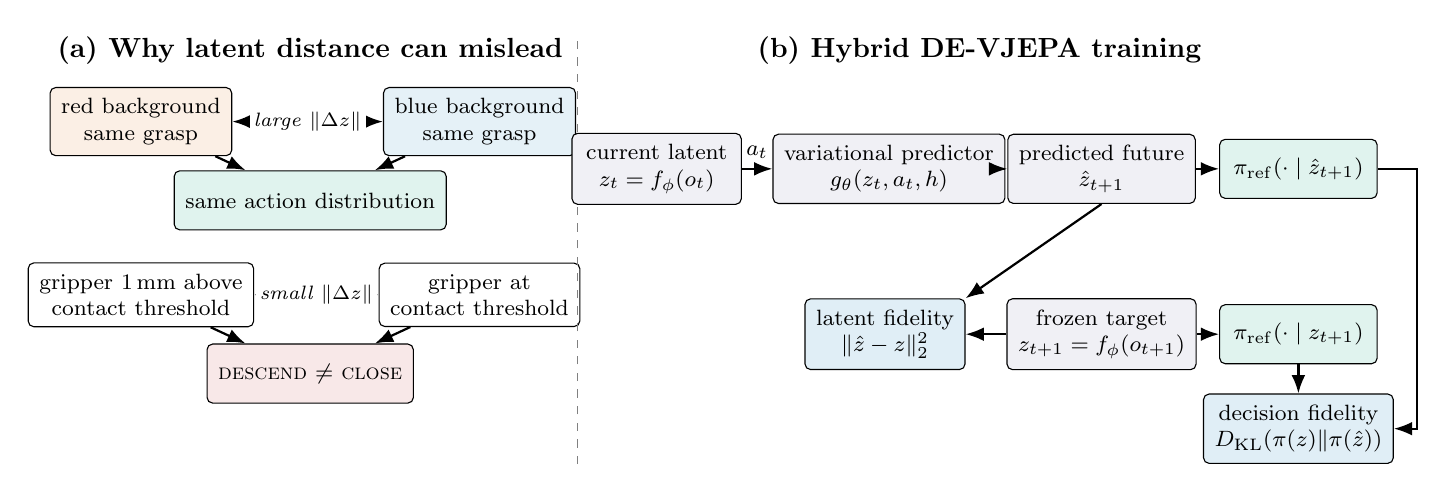
\begin{tikzpicture}[
  font=\footnotesize,
  >=Latex,
  box/.style={draw,rounded corners=2pt,minimum height=0.75cm,align=center,inner sep=4pt},
  state/.style={box,minimum width=2.0cm},
  module/.style={box,minimum width=2.15cm,fill=lightgray},
  policy/.style={box,minimum width=2.0cm,fill=methodgreen!12},
  loss/.style={box,minimum width=2.0cm,fill=methodblue!12},
  arrow/.style={->,thick}
]
  \node[font=\bfseries] at (2.7,3.05) {(a) Why latent distance can mislead};
  \node[state,minimum width=1.7cm,fill=methodorange!10] (texture1) at (0.55,2.15)
    {red background\\same grasp};
  \node[state,minimum width=1.7cm,fill=methodblue!10] (texture2) at (4.85,2.15)
    {blue background\\same grasp};
  \draw[<->,thick] (texture1.east) -- (texture2.west)
    node[midway,fill=white,inner sep=1.5pt,font=\scriptsize\itshape]
    {large $\|\Delta z\|$};
  \node[policy] (sameact) at (2.7,1.15) {same action distribution};
  \draw[arrow] (texture1) -- (sameact);
  \draw[arrow] (texture2) -- (sameact);

  \node[state,minimum width=1.7cm] (above) at (0.55,-0.05) {gripper 1\,mm above\\contact threshold};
  \node[state,minimum width=1.7cm] (contact) at (4.85,-0.05) {gripper at\\contact threshold};
  \draw[<->,thick] (above.east) -- (contact.west)
    node[midway,fill=white,inner sep=1.5pt,font=\scriptsize\itshape]
    {small $\|\Delta z\|$};
  \node[policy,fill=alertred!10] (diffact) at (2.7,-1.05)
    {\textsc{descend} $\neq$ \textsc{close}};
  \draw[arrow] (above) -- (diffact);
  \draw[arrow] (contact) -- (diffact);

  \draw[dashed,gray] (6.1,-2.2) -- (6.1,3.25);

  \node[font=\bfseries] at (11.2,3.05) {(b) Hybrid DE-VJEPA training};
  \node[module] (zt) at (7.1,1.55) {current latent\\$z_t=f_\phi(o_t)$};
  \node[module] (pred) at (10.05,1.55) {variational predictor\\$g_\theta(z_t,a_t,h)$};
  \node[module] (zhat) at (12.75,1.55) {predicted future\\$\hat z_{t+1}$};
  \draw[arrow] (zt) -- node[above]{$a_t$} (pred);
  \draw[arrow] (pred) -- (zhat);

  \node[module] (ztrue) at (12.75,-0.55) {frozen target\\$z_{t+1}=f_\phi(o_{t+1})$};
  \node[policy] (pihat) at (15.25,1.55)
    {$\pi_{\rm ref}(\cdot\mid\hat z_{t+1})$};
  \node[policy] (pitrue) at (15.25,-0.55)
    {$\pi_{\rm ref}(\cdot\mid z_{t+1})$};
  \draw[arrow] (zhat) -- (pihat);
  \draw[arrow] (ztrue) -- (pitrue);
  \node[loss] (latentloss) at (10.0,-0.55)
    {latent fidelity\\$\|\hat z-z\|_2^2$};
  \draw[arrow] (zhat.south) -- (latentloss.north east);
  \draw[arrow] (ztrue) -- (latentloss);
  \node[loss] (decisionloss) at (15.25,-1.75)
    {decision fidelity\\$D_{\rm KL}(\pi(z)\|\pi(\hat z))$};
  \draw[arrow] (pihat.east) -- ++(0.5,0) |- (decisionloss.east);
  \draw[arrow] (pitrue) -- (decisionloss);
\end{tikzpicture}
\caption{\textbf{Prediction--action gap and proposed objective.}
(a) Euclidean latent distance can over-penalize decision-irrelevant appearance
changes and under-penalize small state changes that cross an action boundary.
(b) Hybrid DE-VJEPA retains latent prediction while matching the action
distributions induced by predicted and true future latents. The encoder and
reference policy are frozen; only the variational predictor is updated.}
\label{fig:method-overview}
\end{figure*}

% ── 2. Background ──────────────────────────────────────────────────────────────
\section{Background}
\label{sec:background}

\subsection{Latent World Models}

Let $o_t$ denote the observation at time $t$.
An encoder $f_\phi$ maps observations to latent representations $z_t = f_\phi(o_t)$.
A latent predictor $g_\theta$ produces future latents from current latents and actions:
\[
  \hat{z}_{t+k} = g_\theta(z_t,\,a_{t:t+k}).
\]
The standard prediction objective is $\mathcal{L}_{\text{pred}} = d(\hat{z}_{t+k}, z_{t+k})$,
where $d$ is Euclidean or cosine distance.

\subsection{Variational JEPA}
\label{sec:vjepa}

VJEPA \citep{huang2026vjepa} introduces a latent variable $h$ for hidden uncertainty:
\[
  p_\theta(z_{t+k} \mid z_t, a_{t:t+k}) = \int p_\theta(z_{t+k} \mid z_t, a_{t:t+k}, h)\,p(h)\,dh.
\]
With variational posterior $q_\psi(h \mid z_t, a_{t:t+k}, z_{t+k})$ the training objective is
\begin{equation}
  \mathcal{L}_{\text{VJEPA}}
  = \mathbb{E}_{q_\psi}\!\left[-\log p_\theta(z_{t+k} \mid \cdot)\right]
  + \beta\,D_{\mathrm{KL}}\!\left(q_\psi \,\|\, p(h)\right).
  \label{eq:vjepa}
\end{equation}

\subsection{Bisimulation Metrics}
\label{sec:bisim}

Bisimulation \citep{ferns2004metrics} defines state equivalence by behavioral
similarity: states $s,s'$ are bisimilar if they share the same reward and lead to
bisimilar distributions under every action.
Deep bisimulation for control \citep{zhang2020learning} learns an encoder $\phi$
satisfying
\[
  \|\phi(s)-\phi(s')\| \approx |r(s)-r(s')| + \gamma\,W(\phi \circ T(\cdot\mid s),\,\phi \circ T(\cdot\mid s')),
\]
where $W$ is a Wasserstein distance.
Our work is inspired by this but distinct: we apply a \emph{policy-induced} equivalence
to the \emph{predictor} objective in an existing JEPA architecture, without re-designing
the encoder.


\subsection{Related Work and Positioning}
\label{sec:related}

\paragraph{Latent predictive representation learning.}
DE-VJEPA follows the broad JEPA program of learning by predicting in embedding
space rather than pixel space \citep{lecun2022path,assran2023ijepa,bardes2024vjepa}.
Recent work extends this idea from masked images to video and action-conditioned
world modeling \citep{garrido2024iwm,assran2025vjepa2,destrade2026valuejepa}.
This direction is complementary to reconstruction-heavy self-supervised methods
such as masked autoencoders \citep{he2022mae} and to contrastive predictive
learning \citep{oord2018cpc}: our question is not only whether a latent is
predictable, but whether the predicted latent preserves action-relevant decisions.

\paragraph{World models for control.}
Classical latent world models learn compact dynamics for planning or policy
optimization \citep{ha2018worldmodels,hafner2019planet,hafner2020dreamer,
hafner2021dreamerv2,hafner2023dreamerv3}.
More recent scalable model-based agents such as MuZero, TD-MPC, and TD-MPC2
optimize behavior through latent prediction, value estimation, or model-predictive
control rather than direct pixel reconstruction
\citep{schrittwieser2020muzero,hansen2022tdmpc,hansen2024tdmpc2}.
Generative world-model systems such as UniSim, GAIA-1, Genie, and recent robot
world-model surveys emphasize that future prediction is becoming central to
embodied AI \citep{yang2023unisim,hu2023gaia,bruce2024genie,hou2026survey}.
DE-VJEPA differs by asking how the \emph{training metric} for a world model should
be aligned with downstream decision making.

\paragraph{Robot policies and imitation learning.}
Our use of a frozen behavior-cloned policy is motivated by the practical success
of imitation and visuomotor policy learning, including diffusion policies,
robotics transformers, vision-language-action models, and action-chunking
transformers \citep{ross2011dagger,chi2023diffusionpolicy,brohan2022rt1,
zitkovich2023rt2,zhao2023act}.
At the same time, imitation policies are known to suffer from compounding errors
and distribution shift \citep{ross2011dagger}, which motivates our emphasis on
reference-policy quality, independent evaluator policies, and uncertainty-aware
policy geometry. Cornell-related robot-learning work such as RHyME and X-Sim
similarly highlights the importance of action-relevant alignment under mismatched
demonstrations or embodiments \citep{kedia2024rhyme,dan2025xsim}.

\paragraph{Decision-aware distances and calibration.}
The theoretical side of DE-VJEPA is closest to bisimulation metrics and invariant
representations for control \citep{ferns2004metrics,ferns2011continuous,
zhang2020learning}. It is also related to metric learning: rather than assuming
Euclidean latent distance is meaningful, we learn or impose a task-dependent
geometry \citep{weinberger2009lmnn}. The reference-policy risk is connected to
neural-network calibration, where modern networks can output poorly calibrated
probabilities even when accurate \citep{guo2017calibration}. This motivates the
uncertainty-band formulation in Section~\ref{sec:reliable-geometry}.


% ── 3. Prediction--Action Gap ──────────────────────────────────────────────────
\section{The Prediction--Action Gap}
\label{sec:gap}

Representation-space distance $\|\hat{z}-z\|^2$ can be mis-calibrated for control
in two complementary ways.

\begin{remark}[Prediction--action gap]
(i)~Small latent differences may correspond to different optimal actions (the metric
is too lenient).
(ii)~Large latent differences may be decision-irrelevant (the metric is too strict).
A predictor trained only for latent similarity may therefore learn to preserve
statistically predictable but decision-irrelevant information, while failing to
preserve small action-critical distinctions.
\end{remark}

In embodied manipulation, for instance, a~1\,mm gripper-cup distance difference
may change the optimal action from \textsc{close} to \textsc{descend}, while a
large background-texture change is completely irrelevant.
Standard VJEPA treats both equally.

\paragraph{Concrete examples.}
Consider a button-press trajectory. Changing the table texture can move hundreds
of image pixels and therefore shift a generic visual embedding, yet the correct
end-effector command is unchanged. Conversely, immediately before contact, two
frames may differ by only a few pixels while requiring different commands:
continue descending in one state and begin pressing in the other. The first case
is a \emph{false positive} for latent distance; the second is a \emph{false
negative}. Figure~\ref{fig:method-overview} illustrates both cases. The goal of
DE-VJEPA is not to discard latent fidelity, but to reweight prediction errors by
whether they change the policy distribution.

% ── 4. DE-VJEPA ───────────────────────────────────────────────────────────────
\section{Decision-Equivalent Variational JEPA}
\label{sec:devjepa}

\subsection{Decision-Equivalence Distance}

Let $\pi_{\mathrm{ref}}(a \mid z,\ell)$ be a frozen reference policy conditioned on
latent state $z$ and language instruction $\ell$.
Instead of measuring whether the predicted latent $\hat z$ is close to the target
latent $z$ in Euclidean space, we measure whether the two latents induce the same
action distribution under $\pi_{\mathrm{ref}}$:
\begin{equation}
  d_\pi(\hat z,z)
  =
  D_{\mathrm{KL}}\!\left(
  \pi_{\mathrm{ref}}(\cdot \mid z,\ell)
  \,\middle\|\,
  \pi_{\mathrm{ref}}(\cdot \mid \hat z,\ell)
  \right).
  \label{eq:dpi}
\end{equation}
This distance is asymmetric by design. The forward KL penalizes the predictor when
it fails to preserve an action mode that the reference policy assigns high
probability to at the true future latent.

The key distinction from standard latent prediction is that $d_\pi$ does not ask
whether $\hat z$ and $z$ are visually or geometrically identical. It asks whether
they are \emph{decision-equivalent} for the current instruction.

\subsection{Reliability-Aware Policy Geometry}
\label{sec:reliable-geometry}

A practical difficulty is that $\pi_{\mathrm{ref}}$ is usually trained by behavior
cloning on expert demonstrations.
Such policies can be poorly calibrated outside the demonstration distribution, consistent with broader evidence that modern neural networks often require explicit calibration \citep{guo2017calibration}.
This matters because the predictor $g_\theta$ may produce intermediate latents
$\hat z$ that do not lie exactly on the training-data manifold.
In those regions, the gradient from $d_\pi$ may be noisy or even adversarial.

To avoid treating the reference policy as an oracle everywhere, we use a
reliability-aware version of the decision distance:
\begin{equation}
  d_{\pi,\epsilon}(\hat z,z)
  =
  \left[
  D_{\mathrm{KL}}\!\left(
  \pi_{\mathrm{ref}}(\cdot \mid z,\ell)
  \,\middle\|\,
  \pi_{\mathrm{ref}}(\cdot \mid \hat z,\ell)
  \right)
  -
  \epsilon(\hat z,z)
  \right]_+ ,
  \label{eq:banded-dpi}
\end{equation}
where $[x]_+ = \max(x,0)$.
The tolerance $\epsilon(\hat z,z)$ forms a small uncertainty band around the
reference policy's action distribution.
When the policy is confident and the predicted latent lies near the training
support, $\epsilon$ is small and the loss behaves like the original KL.
When the predicted latent is far from the trusted region of $\pi_{\mathrm{ref}}$,
the band prevents the model from overfitting to unreliable policy gradients.

One simple instantiation is
\begin{equation}
  \epsilon(\hat z,z)
  =
  \epsilon_0
  +
  c \left(
  u(\hat z) + u(z)
  \right),
  \label{eq:epsilon}
\end{equation}
where $u(z)$ is an uncertainty score.
In experiments, $u(z)$ can be estimated using policy entropy, ensemble disagreement,
or latent distance to the demonstration manifold.
This modification does not add a new training objective; it only prevents the
decision-equivalence loss from trusting $\pi_{\mathrm{ref}}$ in regions where the
policy geometry is unreliable.

\subsection{DE-VJEPA Objectives}

The pure decision-equivalence objective is
\begin{equation}
\begin{aligned}
  \mathcal{L}_{\mathrm{DE\text{-}VJEPA}}
  &=
  \mathbb{E}_{q_\psi}
  \left[
  d_{\pi,\epsilon}(\hat z_{t+k}, z_{t+k})
  \right]  \\
  &\quad
  + \beta
  D_{\mathrm{KL}}\!\left(
  q_\psi(h \mid z_t,a_{t:t+k},z_{t+k})
  \,\middle\|\,
  p(h)
  \right).
\end{aligned}
\label{eq:devjepa}
\end{equation}
Here $h$ is the latent stochastic variable from VJEPA, and
\[
  \hat z_{t+k}
  \sim
  p_\theta(\cdot \mid z_t,a_{t:t+k},h).
\]
The encoder $f_\phi$ and the reference policy $\pi_{\mathrm{ref}}$ are frozen.
Only the predictor $g_\theta$ and the variational posterior are updated.

Compared with standard VJEPA, the only structural change is the prediction
criterion.
Instead of training the model to reproduce the exact target latent, DE-VJEPA trains
it to preserve the target latent's action-relevant content.

Empirically, replacing latent prediction entirely is unnecessarily destructive to
representation fidelity. We therefore evaluate the hybrid objective
\begin{equation}
  \mathcal{L}_{\mathrm{hybrid}}
  =
  \mathcal{L}_{\mathrm{VJEPA}}
  +
  \lambda\,
  D_{\mathrm{KL}}\!\left(
  \pi_{\mathrm{ref}}(\cdot\mid z_{t+k})
  \,\middle\|\,
  \pi_{\mathrm{ref}}(\cdot\mid \hat z_{t+k})
  \right).
  \label{eq:hybrid}
\end{equation}
The latent term anchors predictions to the learned representation manifold, while
the policy term emphasizes errors that alter the reference policy distribution.
The pure objective in Eq.~\eqref{eq:devjepa} remains a theoretical limiting case.

\subsection{Multi-Step Decision Equivalence}
\label{sec:multistep}

A single-step policy KL captures immediate action consistency, but world models are
ultimately useful because they support multi-step reasoning.
To connect DE-VJEPA more directly to planning, we also define a multi-step extension:
\begin{equation}
  d_{\pi}^{(K)}
  =
  \sum_{j=1}^{K}
  \gamma^{j-1}
  D_{\mathrm{KL}}\!\left(
  \pi_{\mathrm{ref}}(\cdot \mid z_{t+j},\ell)
  \,\middle\|\,
  \pi_{\mathrm{ref}}(\cdot \mid \hat z_{t+j},\ell)
  \right).
  \label{eq:multistep-dpi}
\end{equation}
This objective asks the predictor to preserve the sequence of future decisions,
not merely the next decision.
The single-step version is still meaningful as a first stage: if a downstream
planner re-queries $\pi_{\mathrm{ref}}$ or another policy at every imagined rollout
step, then local decision consistency at each predicted state is already useful.
However, for long-horizon planning, Eq.~\eqref{eq:multistep-dpi} is the more direct
objective.

A value-based alternative is
\begin{equation}
  d_V(\hat z,z)
  =
  \left|
  V^{\pi_{\mathrm{ref}}}(\hat z,\ell)
  -
  V^{\pi_{\mathrm{ref}}}(z,\ell)
  \right|,
  \label{eq:value-distance}
\end{equation}
which compares predicted and true latents by their estimated long-run value.
We treat $d_V$ as an important ablation rather than the default objective, because
accurate value estimation is harder than estimating a local policy distribution.

\paragraph{Relationship to bisimulation.}
DE-VJEPA is inspired by bisimulation but does not claim to implement full
bisimulation.
Classical bisimulation compares reward and transition structure.
DE-VJEPA instead compares the action distributions induced by a frozen policy.
Thus, it is better understood as a policy-induced behavioral equivalence relation:
two latents are equivalent when they lead the agent to make the same decision.

% ── 5. Theory ─────────────────────────────────────────────────────────────────
\section{Theoretical Motivation}
\label{sec:theory}

\subsection{Policy-Equivalence Classes}

The correct theoretical object in DE-VJEPA is not injectivity of
$\pi_{\mathrm{ref}}$.
In practice, many different latents should induce the same action distribution.
For example, two visually different backgrounds may require exactly the same robot
action.
Therefore, DE-VJEPA should not be interpreted as recovering the true latent state.
It should be interpreted as recovering the true latent state up to
\emph{policy equivalence}.

\begin{definition}[Policy equivalence]
For a fixed instruction $\ell$, define
\[
  z \sim_\pi z'
  \quad \Longleftrightarrow \quad
  \pi_{\mathrm{ref}}(\cdot \mid z,\ell)
  =
  \pi_{\mathrm{ref}}(\cdot \mid z',\ell).
\]
The equivalence class of $z$ is
\[
  [z]_\pi
  =
  \left\{
  z' :
  z' \sim_\pi z
  \right\}.
\]
\end{definition}

\begin{proposition}[Collapse characterization]
\label{prop:collapse}
For any two latents $z$ and $\hat z$,
\[
  d_\pi(\hat z,z) = 0
  \quad \Longleftrightarrow \quad
  \hat z \in [z]_\pi .
\]
Therefore, DE-VJEPA collapses exactly those latent distinctions that are invisible
to the reference policy.
\end{proposition}

\begin{proof}
By the non-negativity of KL divergence,
  $D_{\mathrm{KL}}(p \| q) = 0$
iff $p=q$ almost everywhere.
Applying this to
\[
  p = \pi_{\mathrm{ref}}(\cdot \mid z,\ell),
  \qquad
  q = \pi_{\mathrm{ref}}(\cdot \mid \hat z,\ell),
\]
we obtain
\[
  d_\pi(\hat z,z)=0
  \quad \Longleftrightarrow \quad
  \pi_{\mathrm{ref}}(\cdot \mid z,\ell)
  =
  \pi_{\mathrm{ref}}(\cdot \mid \hat z,\ell).
\]
By the definition of $\sim_\pi$, this is equivalent to
$\hat z \in [z]_\pi$.
\end{proof}

\begin{corollary}[Injective policy as a special case]
If $\pi_{\mathrm{ref}}(\cdot \mid z,\ell)$ is injective in $z$ over the support of
the predictor, then
\[
  d_\pi(\hat z,z)=0
  \quad \Longleftrightarrow \quad
  \hat z=z .
\]
Thus, exact latent recovery is a special case of DE-VJEPA, not the general goal.
\end{corollary}

\begin{remark}[Why non-injectivity is desirable]
A highly expressive policy will not be globally injective.
In low-entropy regions, many latents may map to the same high-confidence action.
This is not a failure of DE-VJEPA.
It is the intended behavior: the model should not waste predictive capacity on
state differences that do not change the decision.
The risk is not non-injectivity itself, but \emph{wrong} non-injectivity, where
$\pi_{\mathrm{ref}}$ collapses states that a better policy would distinguish.
This is why reference-policy quality and uncertainty calibration are central
empirical questions.
\end{remark}

\subsection{When Can DE-VJEPA Fail?}

The collapse characterization also identifies the main failure mode.
If the reference policy ignores a task-critical feature, then DE-VJEPA will also
ignore that feature.
Formally, if there exist two latents $z$ and $z'$ such that
\[
  \pi_{\mathrm{ref}}(\cdot \mid z,\ell)
  =
  \pi_{\mathrm{ref}}(\cdot \mid z',\ell)
\]
but the optimal policy satisfies
\[
  \pi^*(\cdot \mid z,\ell)
  \neq
  \pi^*(\cdot \mid z',\ell),
\]
then DE-VJEPA will incorrectly treat $z$ and $z'$ as equivalent.
This makes the quality of $\pi_{\mathrm{ref}}$ not merely an implementation detail,
but a core assumption of the method.

% ── 6. Experiments ─────────────────────────────────────────────────────────────
\section{Experiments}
\label{sec:experiments}

\subsection{Setup}

We use 33,016 frames from 500 successful demonstrations across five MetaWorld
tasks \citep{yu2020metaworld}: \textsc{reach}, \textsc{button-press},
\textsc{drawer-open}, \textsc{door-open}, and \textsc{pick-place}.
The visual encoder is a frozen ImageNet ResNet-18 proxy, not an official V-JEPA
backbone. We train Gaussian behavior-cloned policies and variational one-step
latent predictors with seeds 42, 1000, and 10000.

\paragraph{Leakage-free evaluation.}
The true future latent is never provided to the predictor at evaluation time.
Each trained predictor is evaluated by policies trained with seeds different from
its training reference policy, producing six source/evaluator-policy pairs.
We report raw latent MSE, independent forward decision KL, and independent
action-mean MSE on clean observations and deterministic brightness, blur, and
desaturation shifts. Statistical tests pair methods by source/evaluator pair.

\subsection{Pilot Reproduction}

At $\lambda=0.01$, clean latent MSE increases by 15.4\%
($p=2.2{\times}10^{-18}$), while independent decision KL and action MSE decrease
by 19.8\% ($p=6.5{\times}10^{-14}$) and 9.0\% ($p=0.0028$). Under brightness,
decision KL decreases by 23.6\% ($p=0.0023$) with no latent-MSE change
($p=0.608$). Figure~\ref{fig:offline-main} summarizes the complete pattern.

\begin{figure*}[t]
\centering
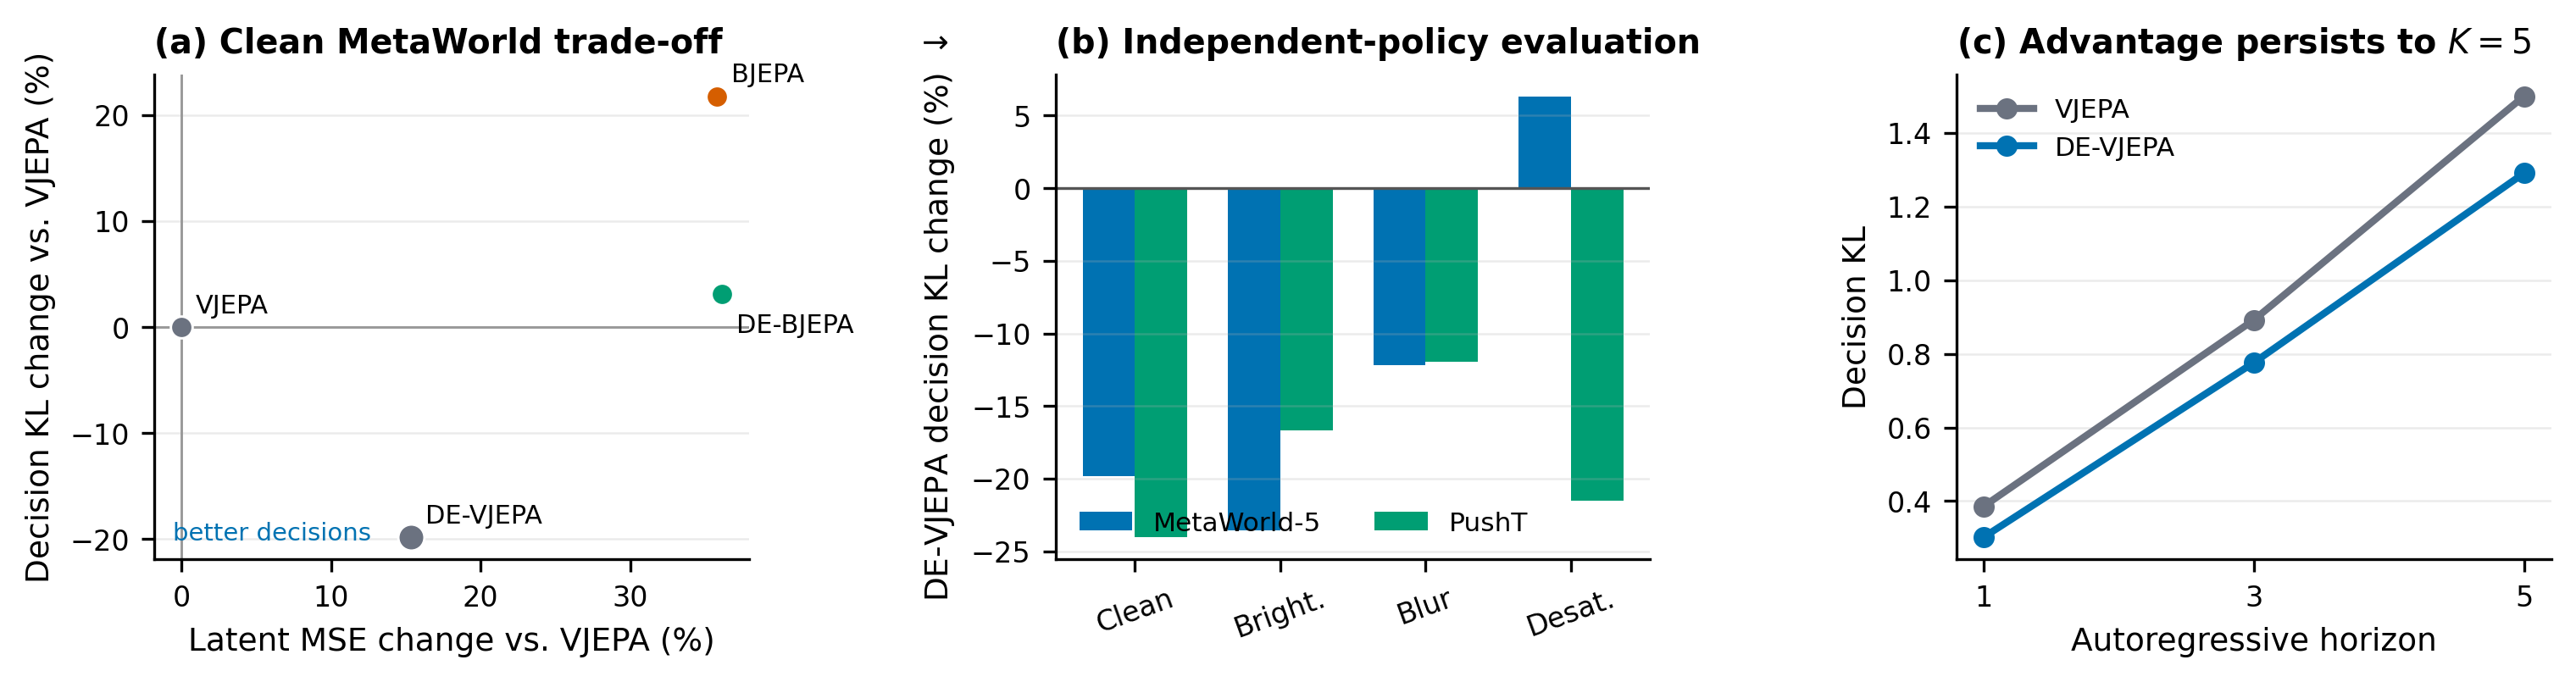
\includegraphics[width=\textwidth]{plots/paper_offline_results.png}
\caption{\textbf{Offline prediction--action results.}
(a) On clean MetaWorld observations, DE-VJEPA moves into the lower-right quadrant:
decision KL improves even though latent MSE worsens. BJEPA shows the opposite
trade-off. (b) Relative to matched VJEPA predictors, DE-VJEPA lowers independent
decision KL in seven of eight dataset--condition comparisons; MetaWorld
desaturation is the exception. Percentages are computed from the paired
DE-VJEPA/VJEPA means. (c) In held-out autoregressive rollouts, the decision-KL
advantage remains visible through horizon five.}
\label{fig:offline-main}
\end{figure*}

\subsection{Lambda Trade-off}

We sweep $\lambda$ over six values on three tasks. The best clean compromise is
$10^{-3}$: decision KL and action MSE fall by 12.6\% and 6.0\%, while latent MSE
rises by 0.9\%. Larger weights eventually degrade all clean metrics
(Figure~\ref{fig:ablation-statistics}a).

\subsection{Does Meaningful Policy Geometry Matter?}

Random policy KL is indistinguishable from baseline; weak BC changes decision KL
by only $-0.26\%$ clean and $-3.81\%$ under brightness. Strong BC produces the
large gains (Figure~\ref{fig:policy-geometry}).

\begin{figure}[t]
\centering
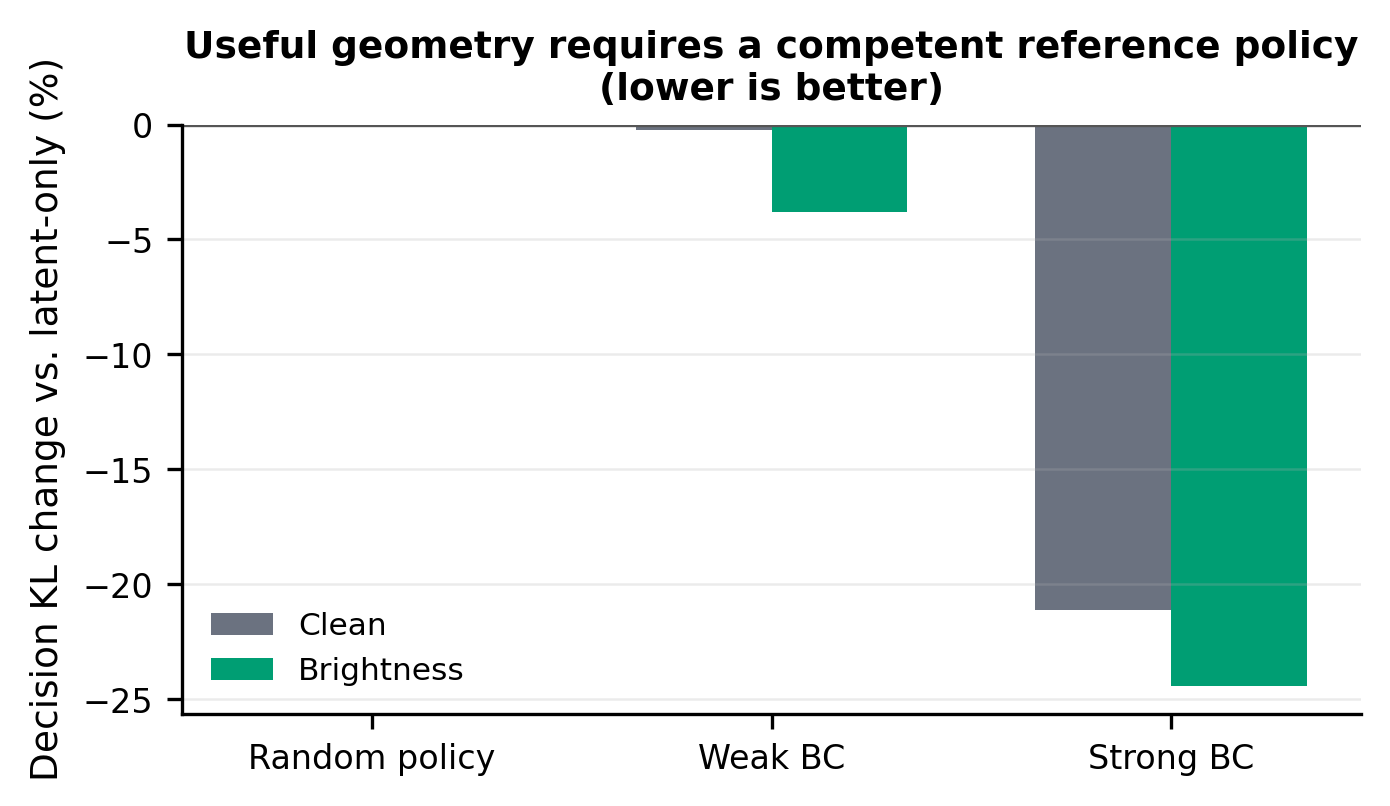
\includegraphics[width=\columnwidth]{plots/paper_policy_geometry.png}
\caption{\textbf{Reference-policy quality ablation.}
Random geometry produces no measurable benefit, weak behavior cloning produces
only a small shift, and strong behavior cloning produces the decision-KL
reduction. This negative control argues against interpreting the auxiliary KL as
generic regularization.}
\label{fig:policy-geometry}
\end{figure}

\subsection{Policy KL Versus Action-Mean Matching}

We compare policy KL with the simpler regularizer
$\|\mu_{\mathrm{ref}}(z)-\mu_{\mathrm{ref}}(\hat z)\|^2$, sweeping its weight from
$10^{-4}$ to $10^{-1}$. Even at its strongest weight, mean matching reduces clean
decision KL by only 3.3\% and is ineffective under brightness; policy KL reduces
the same metrics by 21.1\% and 24.4\%
(Figure~\ref{fig:ablation-statistics}b).

\begin{figure*}[t]
\centering
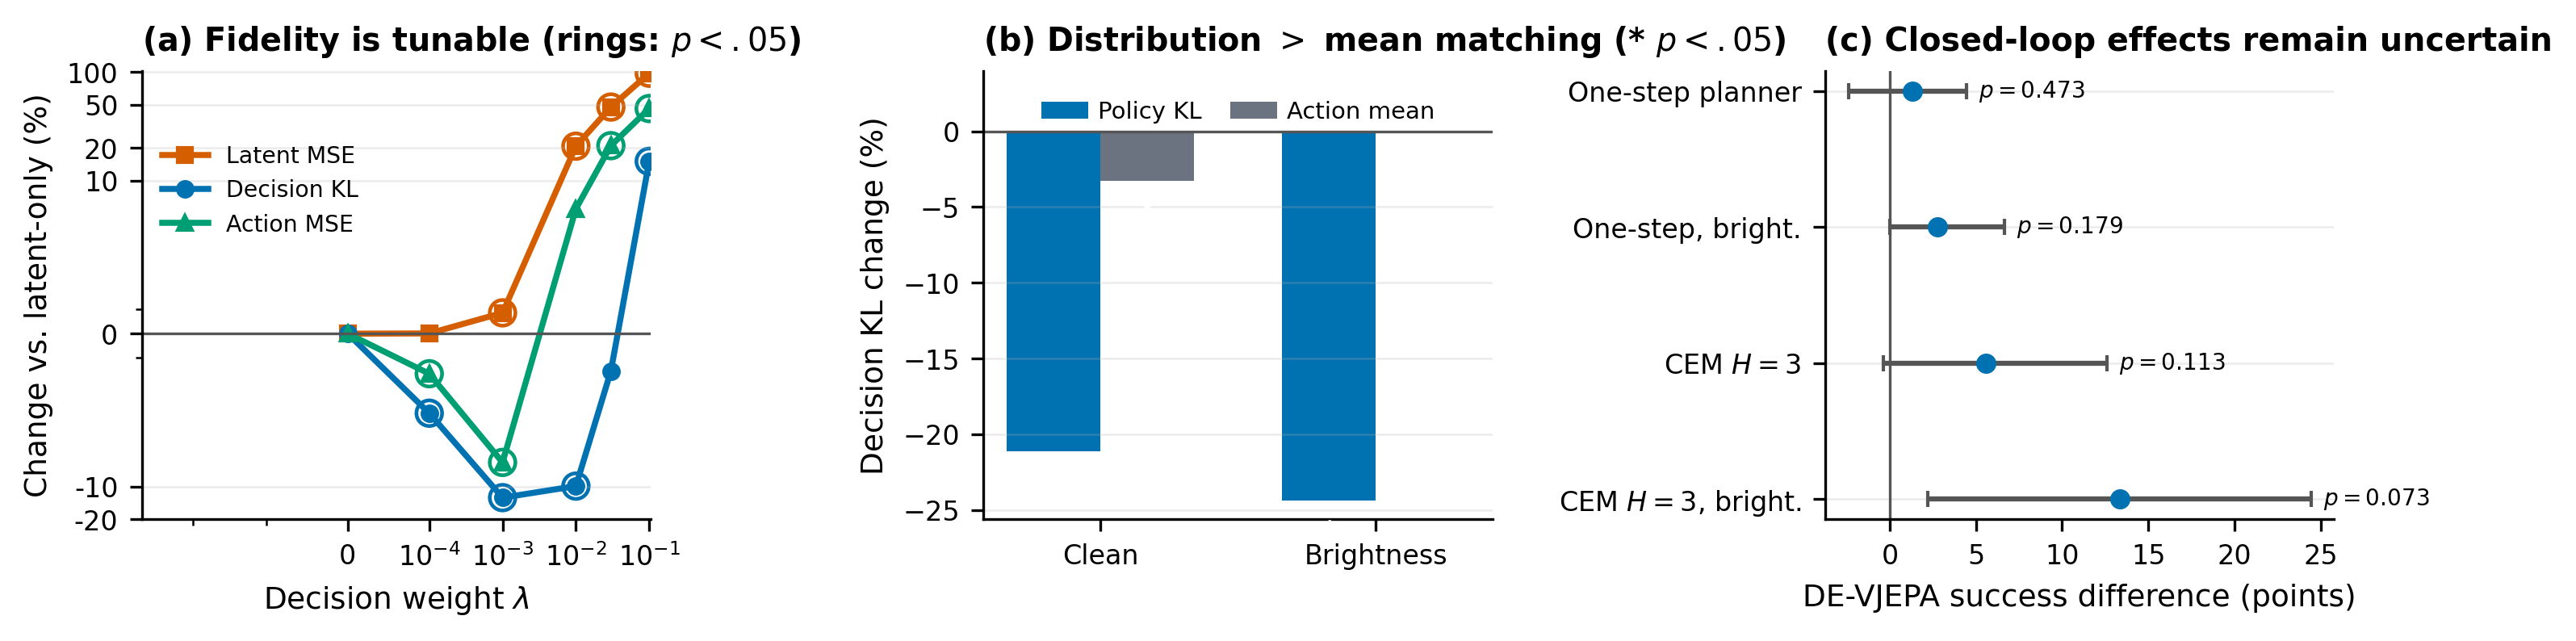
\includegraphics[width=\textwidth]{plots/paper_ablation_statistics.png}
\caption{\textbf{Ablation and inferential-statistics dashboard.}
(a) Clean-data effect sizes across the decision-loss weight; rings mark paired
$p<0.05$. (b) Full-distribution KL is substantially stronger than matching only
the Gaussian policy mean. (c) Closed-loop success differences with paired
bootstrap 95\% confidence intervals. Positive point estimates do not exclude
zero, although the horizon-three brightness result is suggestive.}
\label{fig:ablation-statistics}
\end{figure*}

\subsection{Bayesian Product-of-Experts Extension}

We additionally compare VJEPA and DE-VJEPA with BJEPA and DE-BJEPA. BJEPA combines
a learned diagonal-Gaussian dynamics expert with an empirical task-conditioned
Gaussian prior using a Product of Experts (PoE). The prior is fitted only on
training latents and never observes the held-out future latent.

\begin{table}[t]
\centering
\caption{VJEPA/BJEPA comparison. Values are mean $\pm$ standard error across
30 task/source/evaluator units. Lower is better.}
\label{tab:bjepa-main}
\small
\setlength{\tabcolsep}{3pt}
\resizebox{\columnwidth}{!}{%
\begin{tabular}{@{}llrrr@{}}
\toprule
\textbf{Shift} & \textbf{Method} & \textbf{Latent MSE} &
\textbf{Decision KL} & \textbf{Action MSE} \\
\midrule
Clean & VJEPA & $.00151\pm.00007$ & $.350\pm.024$ & $.000734\pm.000130$ \\
 & BJEPA & $.00205\pm.00014$ & $.426\pm.023$ & $.001000\pm.000159$ \\
 & DE-VJEPA & $.00174\pm.00007$ & $\mathbf{.280\pm.021}$ &
$\mathbf{.000668\pm.000112}$ \\
 & DE-BJEPA & $.00205\pm.00015$ & $.361\pm.021$ & $.000932\pm.000149$ \\
\midrule
Brightness & VJEPA & $.05121\pm.00059$ & $308.5\pm66.4$ & $.07941\pm.00573$ \\
 & BJEPA & $.04878\pm.00074$ & $215.5\pm41.9$ & $.07248\pm.00534$ \\
 & DE-VJEPA & $.05113\pm.00062$ & $235.8\pm52.8$ & $.07436\pm.00546$ \\
 & DE-BJEPA & $\mathbf{.04731\pm.00073}$ & $\mathbf{206.2\pm38.4}$ &
$\mathbf{.07089\pm.00512}$ \\
\bottomrule
\end{tabular}
}
\end{table}

The Bayesian extension is shift-dependent. DE-VJEPA is best on clean decision
KL; DE-BJEPA is best on all three brightness metrics; BJEPA is best on blur
decision KL. None improves desaturated decision KL. Thus uncertainty modeling is
complementary, not uniformly superior.

\subsection{Cross-Dataset Baseline Study}

We next run a matched 11-condition comparison on both the five-task MetaWorld
archive and LeRobot PushT. In addition to VJEPA, BJEPA, DE-VJEPA, and DE-BJEPA,
the matrix includes persistence, linear action-conditioned dynamics, a no-action
predictor, cosine latent prediction, direct action-mean matching, random-policy
KL, and weak-BC-policy KL. PushT contains 25,650 frames from 206 episodes at
10\,Hz. Its two-dimensional actions are absolute pixel targets, which we map from
the $[0,512]$ workspace to $[-1,1]$ before BC training.

\begin{table}[t]
\centering
\caption{DE-VJEPA change relative to VJEPA in the matched cross-dataset study.
Negative values are improvements.}
\label{tab:cross-dataset}
\small
\setlength{\tabcolsep}{3pt}
\resizebox{\columnwidth}{!}{%
\begin{tabular}{@{}llrrr@{}}
\toprule
\textbf{Dataset} & \textbf{Shift} & \textbf{Latent MSE} &
\textbf{Decision KL} & \textbf{Action MSE} \\
\midrule
MetaWorld-5 & Clean & $+15.4\%$ & $\mathbf{-19.8\%}$ & $\mathbf{-9.0\%}$ \\
 & Brightness & $-0.2\%$ & $\mathbf{-23.6\%}$ & $\mathbf{-6.4\%}$ \\
 & Blur & $+1.1\%$ & $\mathbf{-12.2\%}$ & $-0.9\%$ \\
 & Desaturation & $+1.4\%$ & $+6.3\%$ & $+0.8\%$ \\
\midrule
PushT & Clean & $\mathbf{-3.5\%}$ & $\mathbf{-24.0\%}$ & $\mathbf{-13.7\%}$ \\
 & Brightness & $+1.1\%$ & $\mathbf{-16.7\%}$ & $\mathbf{-8.4\%}$ \\
 & Blur & $\mathbf{-1.6\%}$ & $\mathbf{-11.9\%}$ & $\mathbf{-5.1\%}$ \\
 & Desaturation & $+0.6\%$ & $\mathbf{-21.5\%}$ & $\mathbf{-12.0\%}$ \\
\bottomrule
\end{tabular}%
}
\end{table}

Decision KL improves in seven of eight cells. All four PushT paired tests are
significant ($p\leq0.014$), but PushT has only six source/evaluator pairs.
Persistence remains best on clean PushT, so the defensible claim is improvement
over trained VJEPA rather than universal dominance.

\subsection{Extended Baseline Matrix}

\begin{figure*}[t]
\centering
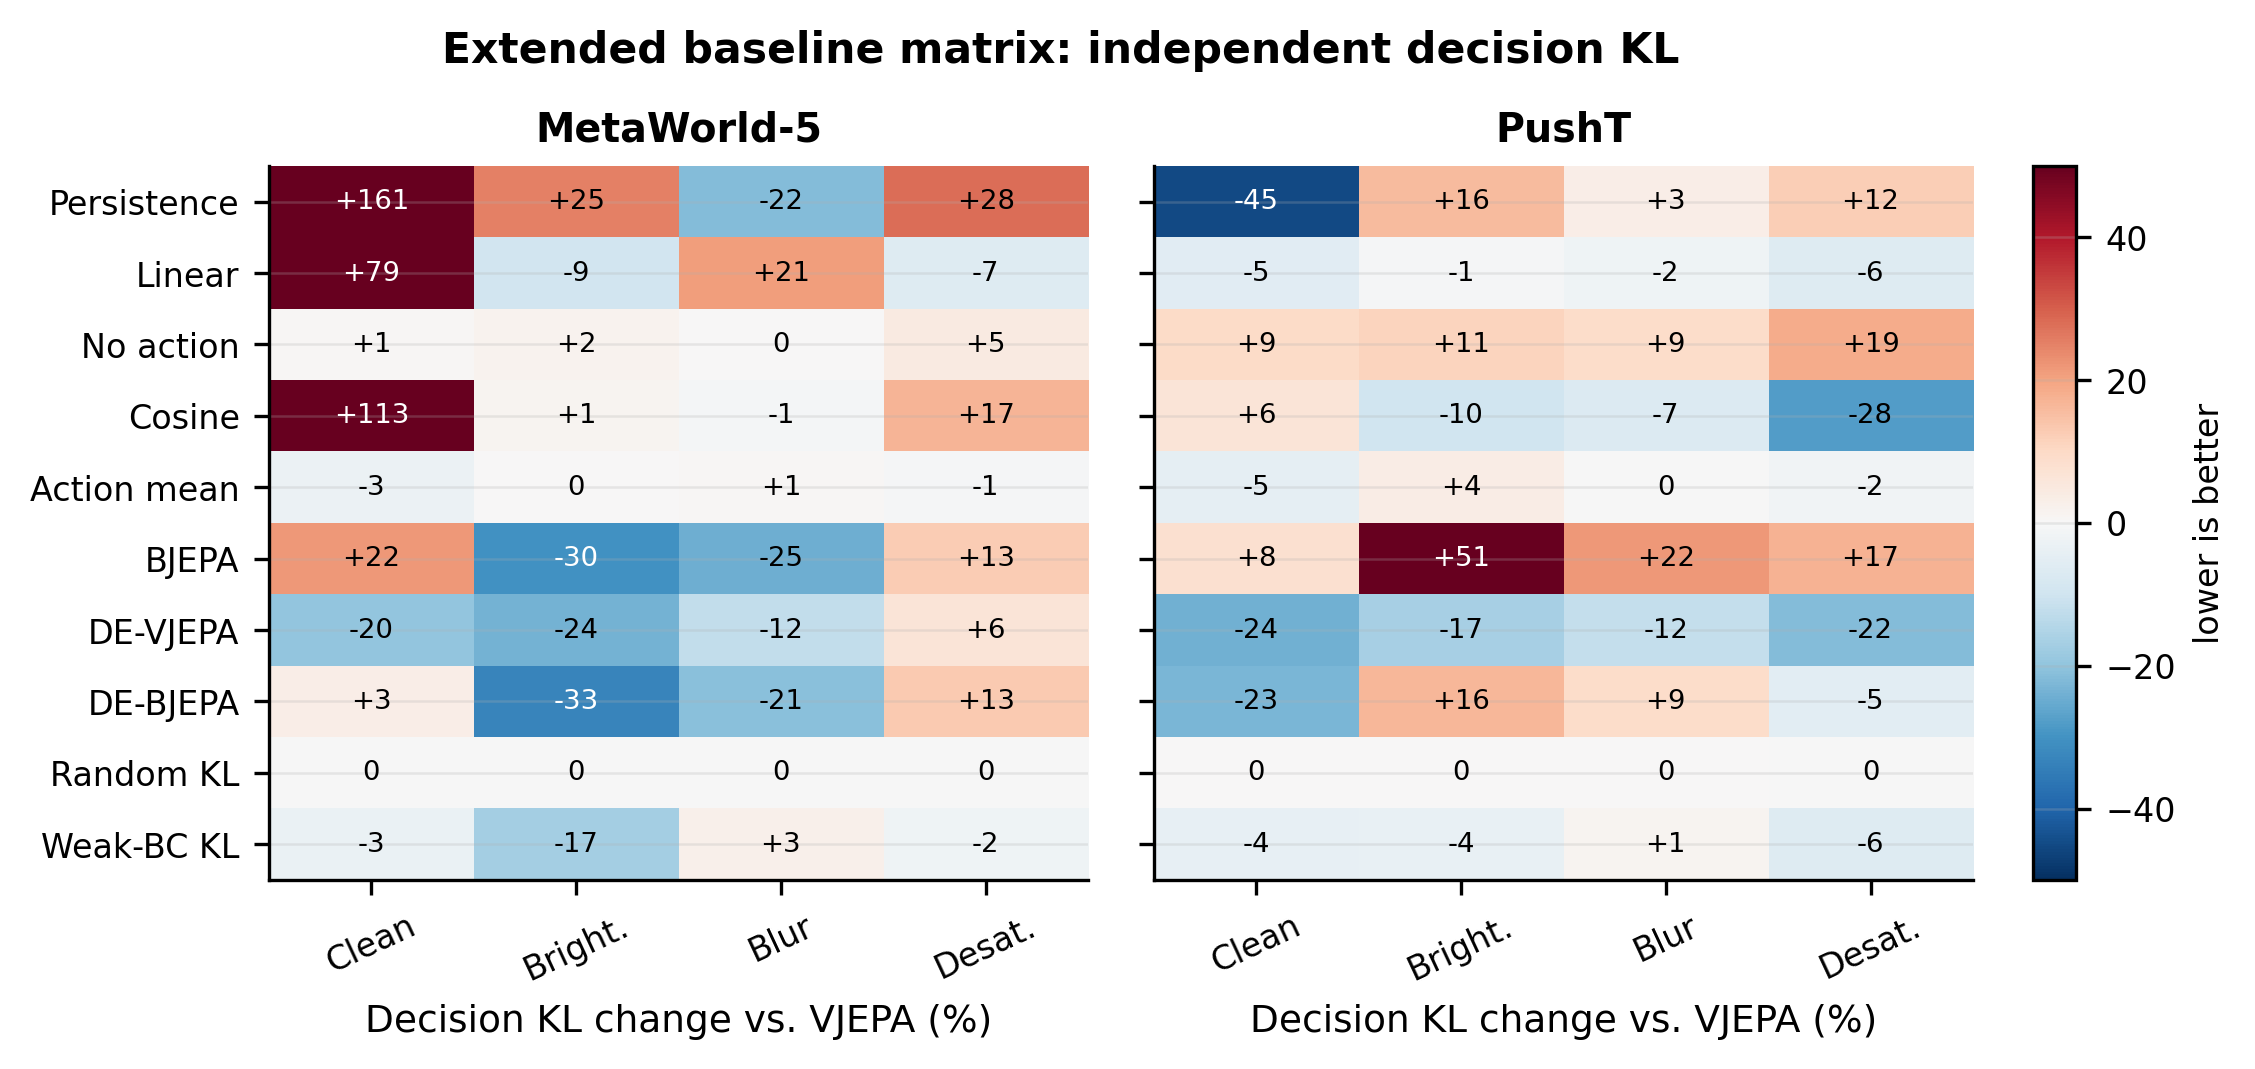
\includegraphics[width=0.86\textwidth]{plots/paper_baseline_heatmap.png}
\caption{\textbf{Ten-method decision-KL matrix.}
Each cell is the percentage change from VJEPA; blue is better. DE-VJEPA is the
only learned nonlinear predictor with improvements in seven of eight
dataset--condition cells. Persistence and cosine prediction win isolated PushT
cells, while BJEPA variants are strongest for selected MetaWorld shifts. Values
are clipped to $\pm50\%$ for color scaling but printed without clipping.}
\label{fig:baseline-heatmap}
\end{figure*}

Figure~\ref{fig:baseline-heatmap} replaces a winner-take-all summary with the
full effect-size matrix. It shows both DE-VJEPA's consistency and the important
exceptions: persistence on clean PushT, cosine prediction under PushT
desaturation, and Bayesian variants under MetaWorld brightness or blur.

\subsection{Closed-Loop MetaWorld Evaluation}
\label{sec:closed-loop}

We evaluate 1,620 episodes over three tasks, three predictor seeds, three visual
conditions, and 20 matched episodes per cell. A seed-7 BC policy, independent of
predictor training, either acts directly or scores 32 one-step candidate actions
using predicted policy entropy. Full planner details are in
Appendix~\ref{app:closed-loop-record}.

\begin{figure}[t]
\centering
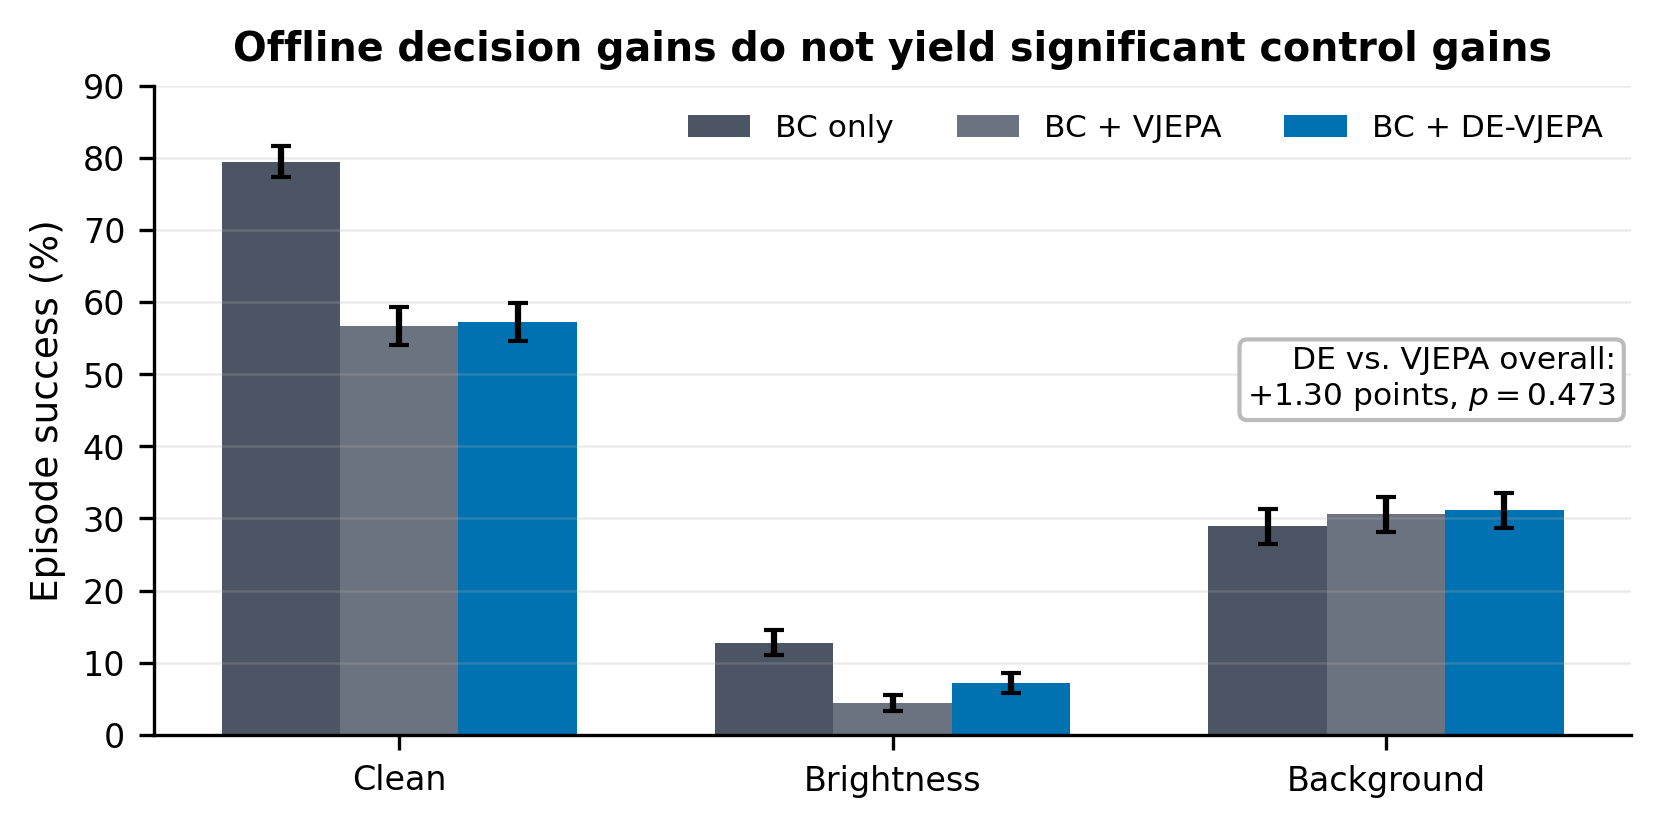
\includegraphics[width=\columnwidth]{plots/paper_closed_loop.png}
\caption{\textbf{Closed-loop transfer.}
Direct BC is strongest on clean observations. DE-VJEPA is directionally better
than VJEPA in aggregate, but the paired difference is not significant. Error
bars are binomial standard errors over 180 episodes per method and condition.}
\label{fig:closed-loop-success}
\end{figure}

DE-VJEPA exceeds VJEPA by 1.30 success points overall
($p=0.473$, 95\% CI $[-2.41,4.44]$) and 2.78 points under brightness
($p=0.179$); neither is significant. BC-only remains 22.22 points stronger on
clean observations. Across a further 13,230 episodes, no local or progress-aware
planner establishes a significant aggregate advantage. The strongest directional
result is CEM at $H=3$ under brightness: $+13.33$ points
($p=0.073$, CI $[2.22,24.44]$). Figure~\ref{fig:ablation-statistics}c displays
the principal confidence intervals.

\section{Discussion}
\label{sec:discussion}

\paragraph{What the experiments establish.}
The central empirical result is metric decoupling: a predictor can become worse
under Euclidean latent error while becoming better under independently evaluated
policy behavior. The effect appears across two datasets and persists in
autoregressive rollouts. The strong/weak/random reference-policy ordering further
shows that the gain depends on meaningful action geometry.

\paragraph{What they do not establish.}
Lower policy KL is not itself a control objective. The closed-loop experiments
show that local entropy, action-consistency, and trajectory-progress scores do not
reliably turn more decision-faithful predictions into better actions. In
particular, planners that deviate from the BC mean can lose more from action
selection error than they gain from improved prediction. DE-VJEPA should therefore
be viewed as a world-model objective whose control value depends on a compatible
value or planning objective, not as a complete model-based controller.

\paragraph{Practical implication.}
Latent MSE alone is insufficient for selecting world models intended for control.
At minimum, evaluation should report both representation error and a held-out
decision metric, preferably using policies not used to define the training loss.
When the two disagree, downstream planning experiments must determine whether the
decision metric captures useful task structure or merely local policy imitation.

% ── 7. Limitations ────────────────────────────────────────────────────────────
\section{Limitations}
\label{sec:limitations}

\paragraph{Reference policy quality.}
$d_\pi$ is only as good as $\pi_{\text{ref}}$.
A poor reference policy may define a decision geometry that ignores task-critical features.

\paragraph{Bias inheritance.}
If $\pi_{\text{ref}}$ ignores certain observations, the world model will too---even
if a better policy would attend to them.

\paragraph{KL direction.}
We use the forward KL; the reverse KL would penalize mode-seeking.
Neither is universally correct; the choice warrants empirical validation.

\paragraph{Continuous action spaces.}
Computing $d_\pi$ exactly requires evaluating KL divergences between continuous
distributions, which is simple for Gaussian policy heads but more difficult for
flow- or diffusion-based policies \citep{chi2023diffusionpolicy}.

\paragraph{Short-horizon limitation.}
Decision equivalence defined via a single-step policy may not capture long-run value.
A natural extension replaces $d_\pi$ with
$d_V(\hat{z}, z) = |V^\pi(\hat{z}) - V^\pi(z)|$.

\paragraph{Empirical scope.}
The offline demonstrations are all successful, so demonstration-level
success correlations are not identifiable, and the ResNet-18 encoder is a
practical proxy rather than a large pretrained video backbone. MetaWorld
contains 30 paired task--training-seed--evaluator-seed units per offline visual
condition, whereas the single-task PushT study contains only six paired
training/evaluator combinations. DE-VJEPA improves offline decision KL over
VJEPA in seven of eight dataset--condition comparisons, but MetaWorld
desaturation is negative and persistence remains stronger on clean PushT.

The closed-loop studies contain 14,850 episodes in total: the original
1,620-episode transfer study, a 4,860-episode local-score ablation, a
4,860-episode one-step progress-planner study, and a 3,510-episode CEM/MPC
study. They cover only three tasks and one independently seeded BC controller.
The learned score is normalized time within successful demonstrations, not
reward-to-go or a true value function. The
background shift is a deterministic image transformation rather than a
physically randomized simulator texture. Neither the local-score planners nor
the progress-aware planners establish a statistically significant aggregate
DE-VJEPA advantage over matched VJEPA, and longer CEM horizons often degrade
clean success. These restrictions preclude claims of general visual
robustness, successful model-based control, or universal superiority.

\iffalse
% Proposal-era feasibility notes retained in source for project history but
% excluded from the submission manuscript.
% ── 8. Feasibility Analysis ───────────────────────────────────────────────────
\section{Feasibility Analysis}
\label{sec:feasibility}

We systematically assess the five most consequential design choices in DE-VJEPA.

\subsection{The Core Hypothesis}

\textbf{Claim:} Latent prediction accuracy and decision quality are genuinely
decoupled often enough to matter.

\medskip
\textbf{Evidence for:}
In the five-task pilot, clean latent MSE becomes 15.6\% worse while independent
decision KL and action MSE improve by 21.1\% and 8.0\%, respectively.
This directly demonstrates that latent and decision fidelity can move in opposite
directions. Prior work on invariant control representations provides complementary
motivation \citep{zhang2020learning}.

\medskip
\textbf{Risk:} For tasks with rich, spatially structured rewards (dense manipulation),
latent accuracy and decision quality may be nearly identical, making the gap
negligible---and the overhead of DE-VJEPA unjustified.

\medskip
\textbf{Assessment:} \textcolor{feasgreen}{\textbf{Supported in the pilot setting.}}
The result establishes metric decoupling, but not improved closed-loop control.

\subsection{Reference Policy as Decision Geometry}

\textbf{Claim:}
A frozen behavior-cloned policy can provide useful local decision geometry, even
when it is not itself a perfect deployment policy.

\medskip
\textbf{Risk:}
This is the most important practical risk in DE-VJEPA.
Behavior-cloned policies are reliable near the demonstration distribution but can
be poorly calibrated on out-of-distribution latents.
The predictor $g_\theta$ may produce exactly such latents during training.
In those regions, the gradient from $d_\pi$ may no longer reflect meaningful action
geometry.
It may instead push the predictor toward artifacts of the reference policy.

\medskip
\textbf{Mitigation and evidence:}
Independent evaluator policies reduce circularity between the training reference
policy and final metrics. The random, weak, and strong policy ablation provides a
direct control: random geometry changes clean decision KL by only $-0.002\%$, weak
BC changes it by $-0.26\%$, and strong BC changes it by $-21.1\%$.
The uncertainty-banded loss in Eq.~\eqref{eq:banded-dpi} remains future work.

\medskip
\textbf{Assessment:}
\textcolor{cautionamber}{\textbf{Moderate risk with positive pilot evidence.}}
The method should not claim that $\pi_{\mathrm{ref}}$ is a universally valid oracle.
The defensible claim is that a well-trained BC policy provides geometry that
transfers to independently seeded evaluators in the tested conditions.

\subsection{KL Divergence Over Continuous Actions}

\textbf{Claim:} $d_\pi = D_{\mathrm{KL}}(\pi_{\text{ref}}(\cdot\mid z) \,\|\, \pi_{\text{ref}}(\cdot\mid\hat{z}))$
can be computed tractably for robot manipulation policies.

\medskip
\textbf{Evidence for:}
MetaWorld and RLBench both use 4--7\,DoF continuous action spaces.
Gaussian policy heads (with diagonal or full covariance) admit closed-form KL
divergence, which is standard in SAC, PPO, and BC implementations.

\medskip
\textbf{Risk:} If $\pi_{\text{ref}}$ is represented as a diffusion policy or a
normalizing flow (increasingly common for dexterous manipulation), closed-form KL
is unavailable. Monte Carlo KL estimation is high-variance and may dominate gradient
noise.

\medskip
\textbf{Assessment:} \textcolor{feasgreen}{\textbf{Tractable for Gaussian policies
(sufficient for MetaWorld/RLBench).}} A note on handling non-Gaussian policies should
appear in the final paper.

\subsection{Policy-Equivalence Characterization}

\textbf{Claim:}
The main theoretical object in DE-VJEPA is not injectivity, but policy equivalence.
The general result, Proposition~\ref{prop:collapse}, requires no injectivity
assumption: it states that DE-VJEPA collapses exactly those latent distinctions
that are invisible to the reference policy.

\medskip
\textbf{Evidence for:}
This matches the intended behavior of the method.
In robot manipulation, many visually different states may require the same action.
For example, changes in background texture, lighting, or irrelevant object details
should not force the world model to predict a different latent if the required
control decision is unchanged.
DE-VJEPA therefore predicts future latents only up to the equivalence class induced
by $\pi_{\mathrm{ref}}$.

\medskip
\textbf{Risk:}
The risk is not non-injectivity itself.
Non-injectivity is desirable when it collapses decision-irrelevant variation.
The real risk is \emph{incorrect collapse}: if $\pi_{\mathrm{ref}}$ assigns the same
action distribution to two states that a better policy would distinguish, then
DE-VJEPA will also treat those states as equivalent.

\medskip
\textbf{Assessment:}
\textcolor{feasgreen}{\textbf{The theoretical framing is sound.}}
Injectivity is only a special-case corollary in which every policy-equivalence
class contains a single latent.
The practically relevant case is the non-injective one, where the method learns
future states up to action-relevant equivalence classes.
The empirical question is whether the equivalence classes induced by
$\pi_{\mathrm{ref}}$ are useful for downstream control.

\subsection{Experimental Scale and Compute}

\textbf{Claim:} The MetaWorld $\to$ RLBench protocol is achievable at research-lab scale.

\medskip
\textbf{Evidence for:}
MetaWorld tasks (45 tasks, 50\,Hz sim) run at $>$10K steps/second on a single GPU.
DreamerV3 and similar world models train competitive MetaWorld agents in $\sim$1--2
days on a single A100. The DE-VJEPA training loop (frozen encoder, frozen policy,
predictor-only updates) is computationally lighter than full world model training.

\medskip
\textbf{Risk:} RLBench requires rendering 128$\times$128 RGBD images and uses
PyRep/CoppeliaSim, which is harder to parallelize.
The KL evaluation per step adds a forward pass through $\pi_{\text{ref}}$, roughly
doubling the predictor training cost.

\medskip
\textbf{Assessment:} \textcolor{feasgreen}{\textbf{Feasible on one consumer GPU
for the reported offline study.}} The completed pilot and ablations used frozen
encodings, Gaussian policies, and predictor-only updates on an RTX~4090. RLBench
and end-to-end closed-loop training require a separate compute assessment; the
reported 1,620-episode closed-loop evaluation also ran on the same RTX~4090.

% ── Summary Table ─────────────────────────────────────────────────────────────
\subsection{Summary}

\begin{table}[ht]
\centering
\caption{Feasibility summary for each design choice.}
\label{tab:feasibility}
\small
\setlength{\tabcolsep}{4pt}
\begin{tabular}{@{}llc@{}}
\toprule
\textbf{Component} & \textbf{Key risk} & \textbf{Rating} \\
\midrule
Core hypothesis       & Gap may be task-dependent    & \textcolor{feasgreen}{$\bullet\bullet\bullet$} \\
Policy geometry       & BC out-of-distribution       & \textcolor{cautionamber}{$\bullet\bullet\circ$} \\
KL computation        & Non-Gaussian policies        & \textcolor{feasgreen}{$\bullet\bullet\bullet$} \\
Policy equivalence    & Wrong collapse by $\pi_{\mathrm{ref}}$ & \textcolor{cautionamber}{$\bullet\bullet\circ$} \\
Experimental scale    & RLBench parallelism          & \textcolor{feasgreen}{$\bullet\bullet\bullet$} \\
\bottomrule
\multicolumn{3}{@{}l@{}}{\footnotesize $\bullet\bullet\bullet$: low risk;
$\bullet\bullet\circ$: moderate risk.}
\end{tabular}
\end{table}
\fi

% ── 9. Conclusion ──────────────────────────────────────────────────────────────
\section{Conclusion}

We proposed hybrid DE-VJEPA, which supplements variational latent prediction with
a policy-induced KL regularizer. It reduces independent decision KL in seven of
eight MetaWorld/PushT conditions, sometimes while latent MSE worsens, and the
effect requires a competent reference policy. The advantage persists through
five-step autoregressive prediction.

The closed-loop evidence is deliberately negative: none of the tested planners
produces a significant aggregate success gain. DE-VJEPA therefore establishes
better \emph{decision preservation}, not yet better control. The remaining
challenge is to pair this geometry with a task-grounded value objective and a
planning horizon matched to model training.

% ── References ────────────────────────────────────────────────────────────────
\bibliographystyle{abbrvnat}
\begin{thebibliography}{99}

\bibitem[Assran et al.(2023)]{assran2023ijepa}
M.~Assran, Q.~Duval, I.~Misra, P.~Bojanowski, P.~Vincent, M.~Rabbat,
Y.~LeCun, and N.~Ballas.
\newblock Self-supervised learning from images with a joint-embedding predictive architecture.
\newblock In \emph{CVPR}, 2023.

\bibitem[Assran et al.(2025)]{assran2025vjepa2}
M.~Assran, A.~Bardes, Q.~Garrido, and others.
\newblock {V-JEPA 2}: Self-supervised video models enable understanding,
prediction and planning.
\newblock \emph{arXiv:2506.09985}, 2025.

\bibitem[Bardes et al.(2024)]{bardes2024vjepa}
A.~Bardes, Q.~Garrido, J.~Ponce, X.~Chen, M.~Rabbat, Y.~LeCun,
M.~Assran, and N.~Ballas.
\newblock Revisiting feature prediction for learning visual representations from video.
\newblock \emph{arXiv:2404.08471}, 2024.

\bibitem[Brohan et al.(2022)]{brohan2022rt1}
A.~Brohan, N.~Brown, J.~Carbajal, Y.~Chebotar, J.~Dabis, C.~Finn,
K.~Gopalakrishnan, K.~Hausman, A.~Herzog, J.~Hsu, and others.
\newblock {RT-1}: Robotics transformer for real-world control at scale.
\newblock \emph{arXiv:2212.06817}, 2022.

\bibitem[Bruce et al.(2024)]{bruce2024genie}
J.~Bruce, M.~Dennis, A.~Edwards, and others.
\newblock Genie: Generative interactive environments.
\newblock \emph{arXiv:2402.15391}, 2024.

\bibitem[Chi et al.(2023)]{chi2023diffusionpolicy}
C.~Chi, Z.~Xu, S.~Feng, E.~Cousineau, Y.~Du, B.~Burchfiel, R.~Tedrake,
and S.~Song.
\newblock Diffusion policy: Visuomotor policy learning via action diffusion.
\newblock In \emph{RSS}, 2023.

\bibitem[Dan et al.(2025)]{dan2025xsim}
P.~Dan, K.~Kedia, A.~Chao, E.~W. Duan, M.~A. Pace, W.-C. Ma, and
S.~Choudhury.
\newblock {X-Sim}: Cross-embodiment learning via real-to-sim-to-real.
\newblock \emph{arXiv:2505.07096}, 2025.

\bibitem[Destrade et al.(2026)]{destrade2026valuejepa}
M.~Destrade and others.
\newblock Value-guided action planning with {JEPA} world models.
\newblock \emph{arXiv:2601.00844}, 2026.

\bibitem[Ferns et al.(2004)]{ferns2004metrics}
N.~Ferns, P.~Panangaden, and D.~Precup.
\newblock Metrics for finite Markov decision processes.
\newblock In \emph{UAI}, pages 162--169, 2004.

\bibitem[Ferns et al.(2011)]{ferns2011continuous}
N.~Ferns, P.~Panangaden, and D.~Precup.
\newblock Bisimulation metrics for continuous Markov decision processes.
\newblock \emph{SIAM Journal on Computing}, 40(6):1662--1714, 2011.

\bibitem[Garrido et al.(2024)]{garrido2024iwm}
Q.~Garrido, M.~Assran, N.~Ballas, A.~Bardes, L.~Najman, and Y.~LeCun.
\newblock Learning and leveraging world models in visual representation learning.
\newblock \emph{arXiv:2403.00504}, 2024.

\bibitem[Guo et al.(2017)]{guo2017calibration}
C.~Guo, G.~Pleiss, Y.~Sun, and K.~Q. Weinberger.
\newblock On calibration of modern neural networks.
\newblock In \emph{ICML}, 2017.

\bibitem[Ha and Schmidhuber(2018)]{ha2018worldmodels}
D.~Ha and J.~Schmidhuber.
\newblock World models.
\newblock \emph{arXiv:1803.10122}, 2018.

\bibitem[Hafner et al.(2019)]{hafner2019planet}
D.~Hafner, T.~Lillicrap, I.~Fischer, R.~Villegas, D.~Ha, H.~Lee, and
J.~Davidson.
\newblock Learning latent dynamics for planning from pixels.
\newblock In \emph{ICML}, 2019.

\bibitem[Hafner et al.(2020)]{hafner2020dreamer}
D.~Hafner, T.~Lillicrap, J.~Ba, and M.~Norouzi.
\newblock Dream to control: Learning behaviors by latent imagination.
\newblock In \emph{ICLR}, 2020.

\bibitem[Hafner et al.(2021)]{hafner2021dreamerv2}
D.~Hafner, T.~Lillicrap, M.~Norouzi, and J.~Ba.
\newblock Mastering Atari with discrete world models.
\newblock In \emph{ICLR}, 2021.

\bibitem[Hafner et al.(2023)]{hafner2023dreamerv3}
D.~Hafner, J.~Pasukonis, J.~Ba, and T.~Lillicrap.
\newblock Mastering diverse domains through world models.
\newblock \emph{arXiv:2301.04104}, 2023.

\bibitem[Hansen et al.(2022)]{hansen2022tdmpc}
N.~Hansen, X.~Wang, and H.~Su.
\newblock Temporal difference learning for model predictive control.
\newblock In \emph{ICML}, 2022.

\bibitem[Hansen et al.(2024)]{hansen2024tdmpc2}
N.~Hansen, H.~Su, and X.~Wang.
\newblock {TD-MPC2}: Scalable, robust world models for continuous control.
\newblock In \emph{ICLR}, 2024.

\bibitem[He et al.(2022)]{he2022mae}
K.~He, X.~Chen, S.~Xie, Y.~Li, P.~Doll{\'a}r, and R.~Girshick.
\newblock Masked autoencoders are scalable vision learners.
\newblock In \emph{CVPR}, 2022.

\bibitem[Hou et al.(2026)]{hou2026survey}
B.~Hou, G.~Li, J.~Jia, T.~An, X.~Guo, S.~Leng, H.~Geng, Y.~Ze,
T.~Harada, P.~Torr, O.~Mees, M.~Pollefeys, Z.~Liu, J.~Wu,
P.~Abbeel, J.~Malik, Y.~Du, and J.~Yang.
\newblock World model for robot learning: A comprehensive survey.
\newblock \emph{arXiv:2605.00080}, 2026.

\bibitem[Hu et al.(2023)]{hu2023gaia}
A.~Hu, L.~Russell, H.~Yeo, Z.~Murez, G.~Fedoseev, A.~Kendall,
J.~Shotton, and G.~Corrado.
\newblock {GAIA-1}: A generative world model for autonomous driving.
\newblock \emph{arXiv:2309.17080}, 2023.

\bibitem[Huang(2026)]{huang2026vjepa}
Y.~Huang.
\newblock {VJEPA}: Variational joint embedding predictive architectures as
probabilistic world models.
\newblock \emph{arXiv:2601.14354}, 2026.

\bibitem[James et al.(2020)]{james2020rlbench}
S.~James, Z.~Ma, D.~R. Arrojo, and A.~J. Davison.
\newblock {RLBench}: The robot learning benchmark \& learning environment.
\newblock \emph{IEEE RA-L}, 5(2):3019--3026, 2020.

\bibitem[Kedia et al.(2024)]{kedia2024rhyme}
K.~Kedia, P.~Dan, A.~Chao, M.~A. Pace, and S.~Choudhury.
\newblock One-shot imitation under mismatched execution.
\newblock \emph{arXiv:2409.06615}, 2024.

\bibitem[LeCun(2022)]{lecun2022path}
Y.~LeCun.
\newblock A path towards autonomous machine intelligence.
\newblock OpenReview, 2022.

\bibitem[Mao et al.(2025)]{mao2025physworld}
J.~Mao, S.~He, H.-N. Wu, Y.~You, S.~Sun, Z.~Wang, Y.~Bao, H.~Chen,
L.~Guibas, V.~Guizilini, H.~Zhou, and Y.~Wang.
\newblock Robot learning from a physical world model.
\newblock \emph{arXiv:2511.07416}, 2025.

\bibitem[Oord et al.(2018)]{oord2018cpc}
A.~van~den Oord, Y.~Li, and O.~Vinyals.
\newblock Representation learning with contrastive predictive coding.
\newblock \emph{arXiv:1807.03748}, 2018.

\bibitem[Ross et al.(2011)]{ross2011dagger}
S.~Ross, G.~Gordon, and D.~Bagnell.
\newblock A reduction of imitation learning and structured prediction to no-regret online learning.
\newblock In \emph{AISTATS}, 2011.

\bibitem[Schrittwieser et al.(2020)]{schrittwieser2020muzero}
J.~Schrittwieser, I.~Antonoglou, T.~Hubert, and others.
\newblock Mastering Atari, Go, chess and shogi by planning with a learned model.
\newblock \emph{Nature}, 588:604--609, 2020.

\bibitem[Weinberger and Saul(2009)]{weinberger2009lmnn}
K.~Q. Weinberger and L.~K. Saul.
\newblock Distance metric learning for large margin nearest neighbor classification.
\newblock \emph{Journal of Machine Learning Research}, 10:207--244, 2009.

\bibitem[Yang et al.(2023)]{yang2023unisim}
S.~Yang, J.~Walker, J.~Parker-Holder, and others.
\newblock Learning interactive real-world simulators.
\newblock \emph{arXiv:2310.06114}, 2023.

\bibitem[Yu et al.(2020)]{yu2020metaworld}
T.~Yu, D.~Quillen, Z.~He, R.~Julian, K.~Hausman, C.~Finn, and S.~Levine.
\newblock Meta-world: A benchmark and evaluation for multi-task and meta
reinforcement learning.
\newblock In \emph{CoRL}, 2020.

\bibitem[Zhang et al.(2021)]{zhang2020learning}
A.~Zhang, R.~McAllister, R.~Calandra, Y.~Gal, and S.~Levine.
\newblock Learning invariant representations for reinforcement learning without reconstruction.
\newblock In \emph{ICLR}, 2021.

\bibitem[Zhao et al.(2023)]{zhao2023act}
T.~Z. Zhao, V.~Kumar, S.~Levine, and C.~Finn.
\newblock Learning fine-grained bimanual manipulation with low-cost hardware.
\newblock In \emph{RSS}, 2023.

\bibitem[Zitkovich et al.(2023)]{zitkovich2023rt2}
B.~Zitkovich, T.~Yu, S.~Xu, and others.
\newblock {RT-2}: Vision-language-action models transfer web knowledge to robotic control.
\newblock In \emph{CoRL}, 2023.

\end{thebibliography}

\clearpage
\appendix
\section{Reproducibility Appendix}
\label{app:reproducibility}

\subsection{Dataset and Evaluation Units}

The archive contains 33,016 encoded frames from 500 successful MetaWorld
demonstrations, with 100 episodes for each of \textsc{reach},
\textsc{button-press}, \textsc{drawer-open}, \textsc{door-open}, and
\textsc{pick-place}. Removing transitions that cross episode boundaries gives
32,516 valid one-step prediction examples before splitting. Observations are
rendered at $224\times224$ from the \texttt{corner2} camera and encoded once by a
frozen ImageNet ResNet-18 into 512-dimensional latents. Actions are
four-dimensional continuous MetaWorld controls.

For each seed in $\{42,1000,10000\}$, episodes are shuffled and split 80/20 into
training and validation sets. Splitting is performed by episode rather than by
frame. Each trained predictor is evaluated by the two behavior-cloned evaluator
policies whose seeds differ from its training/reference-policy seed. Consequently,
each visual condition contains
$5$ tasks $\times 3$ training seeds $\times 2$ evaluator seeds $=30$ paired
experimental units. Frame-level metrics are saved, but hypothesis tests first
average frames within each task/source/evaluator unit to avoid treating correlated
frames as independent replicates.

\paragraph{PushT.}
The second dataset is the official LeRobot PushT release
(\url{https://huggingface.co/datasets/lerobot/pusht}). It contains 25,650 frames
from 206 single-task episodes, with $96\times96$ RGB observations,
two-dimensional agent state, and two-dimensional target-position actions at
10\,Hz. We decode the provided AV1 video, retain the published episode indices,
and encode each frame with the same frozen ResNet-18 used for MetaWorld. PushT
actions are pixel coordinates with observed range approximately $[12,511]$; they
are transformed as $a'=a/256-1$ so the bounded Gaussian policy mean can represent
the action domain. An initial unnormalized run caused policy collapse and is
explicitly archived as invalid; none of its metrics is used in the paper.

PushT uses the same three training seeds and two non-matching evaluator seeds per
source seed. Because it has one task, each condition has six paired
source/evaluator units rather than MetaWorld's 30 task/source/evaluator units.

\subsection{Visual Conditions}

Clean evaluation uses the frozen archive without image modification. The three
held-out image transformations are deterministic: brightness is multiplied by
$0.55$, Gaussian blur uses radius $2.0$, and color saturation is multiplied by
$0.15$. The same frame ordering, episode identifiers, actions, and task labels are
retained in every shifted archive, allowing sample-aligned evaluation.

\subsection{Model and Optimization Details}

\begin{table*}[t]
\centering
\caption{Concrete implementation and training configuration used in the reported
four-method comparison.}
\label{tab:implementation-details}
\small
\setlength{\tabcolsep}{5pt}
\begin{tabular}{@{}lll@{}}
\toprule
\textbf{Component} & \textbf{Setting} & \textbf{Details} \\
\midrule
Encoder & Frozen ResNet-18 & ImageNet weights; 512-D latent; no fine-tuning \\
Reference/evaluator policy & Gaussian BC & 2-layer MLP, width 512, SiLU,
32-D task embedding \\
Policy output & Diagonal Gaussian & Tanh mean; log standard deviation clipped
to $[-5,1]$ \\
Policy training & AdamW & 30 epochs, batch 1024, lr $3{\times}10^{-4}$,
weight decay $10^{-5}$ \\
Predictor context & $z_t,a_t,\ell$ & One-step horizon; 32-D task embedding \\
Variational state & Gaussian $h$ & 64 dimensions; log variance clipped to
$[-10,5]$ \\
Predictor network & Residual MLP & 2 hidden layers, width 1024, LayerNorm, SiLU \\
Predictor training & AdamW & 50 epochs, batch 512, lr $3{\times}10^{-4}$,
weight decay $10^{-5}$ \\
Regularization & Gradient clipping & Global norm clipped to $5.0$; AMP enabled \\
VAE weight & $\beta=10^{-3}$ & KL from posterior $q(h\mid z_t,a_t,z_{t+1})$
to standard normal \\
Decision weight & $\lambda_{\mathrm{DE}}=10^{-2}$ & Used by DE-VJEPA and
DE-BJEPA \\
BJEPA prior & Empirical task Gaussian & Per-task mean/variance from normalized
training latents only \\
BJEPA objective & Gaussian NLL & Diagonal predictive NLL plus variational KL \\
Hardware & RTX 4090 & Single 24\,GB GPU; eight data-loader workers \\
\bottomrule
\end{tabular}
\end{table*}

Latents and actions are standardized using statistics fitted only on the training
partition for each seed. The same normalization is stored with each BC checkpoint
and reused by its corresponding predictor. Predictor validation and final
evaluation use deterministic predictive means; stochastic samples are used only
for the variational training path.

\subsection{Product-of-Experts BJEPA}

The dynamics expert predicts diagonal Gaussian parameters
$(\mu_{\mathrm{dyn}},\sigma^2_{\mathrm{dyn}})$ from the current latent, action,
task embedding, and variational state. The prior expert is an empirical diagonal
Gaussian $(\mu_{\mathrm{prior},\ell},\sigma^2_{\mathrm{prior},\ell})$ fitted for
task $\ell$ on training target latents. It does not use $z_{t+1}$ at inference.
The combined prediction is
\begin{align}
\tau_{\mathrm{B}} &= \sigma_{\mathrm{dyn}}^{-2}
                   + \sigma_{\mathrm{prior}}^{-2}, \\
\sigma_{\mathrm{B}}^2 &= \tau_{\mathrm{B}}^{-1}, \\
\mu_{\mathrm{B}} &= \sigma_{\mathrm{B}}^2
\left(\sigma_{\mathrm{dyn}}^{-2}\mu_{\mathrm{dyn}}
+\sigma_{\mathrm{prior}}^{-2}\mu_{\mathrm{prior}}\right).
\end{align}
All operations are elementwise. Log variances are clipped to $[-10,5]$, variances
are lower-bounded by $10^{-6}$ before inversion, and training aborts on non-finite
precision, variance, mean, or loss.

\subsection{Training Algorithm}

\begin{figure*}[t]
\centering
\fbox{\begin{minipage}{0.94\textwidth}
\textbf{Algorithm 1: Leakage-free training and evaluation of VJEPA/BJEPA variants}
\begin{enumerate}[leftmargin=1.6em,itemsep=1pt,topsep=3pt]
  \item Split demonstration episodes into seed-specific training and validation
  partitions; fit latent/action normalization on training data only.
  \item Train a Gaussian BC reference policy on normalized training latents. For
  each source seed, reserve the policies from the other two seeds as evaluators.
  \item For BJEPA variants, fit the task-conditioned empirical Gaussian prior using
  normalized training latents only.
  \item For each minibatch, encode context $(z_t,a_t,\ell)$ and infer
  $q_\psi(h\mid z_t,a_t,z_{t+1},\ell)$ for the variational training path.
  \item Predict $\hat z_{t+1}$. VJEPA uses a residual point predictor; BJEPA
  combines dynamics and task-prior experts with the diagonal Gaussian PoE.
  \item Compute the base loss: latent MSE for VJEPA or predictive Gaussian NLL for
  BJEPA. Add $\beta D_{\mathrm{KL}}(q_\psi(h)\|{\cal N}(0,I))$.
  \item For DE variants, add
  $\lambda_{\mathrm{DE}}D_{\mathrm{KL}}(
  \pi_{\mathrm{ref}}(\cdot\mid z_{t+1})\|
  \pi_{\mathrm{ref}}(\cdot\mid\hat z_{t+1}))$.
  \item Update predictor parameters with AdamW. The encoder and reference policy
  remain frozen.
  \item At evaluation, remove the true future latent from predictor inputs, use
  the predictive mean, and score with independently seeded evaluator policies.
\end{enumerate}
\end{minipage}}
\end{figure*}

\subsection{Complete Four-Method Results}

\begin{table*}[t]
\centering
\caption{Complete core comparison. Entries are mean $\pm$ standard error across
30 paired task/source/evaluator units. Lower is better. Bold denotes the lowest
mean within each shift and metric.}
\label{tab:complete-core-results}
\small
\resizebox{\textwidth}{!}{%
\begin{tabular}{@{}llrrr@{}}
\toprule
\textbf{Shift} & \textbf{Method} & \textbf{Latent MSE} &
\textbf{Decision KL} & \textbf{Action MSE} \\
\midrule
Clean & VJEPA & $\mathbf{0.001506\pm0.000067}$ & $0.3496\pm0.0237$ &
$0.000734\pm0.000130$ \\
 & BJEPA & $0.002045\pm0.000145$ & $0.4257\pm0.0230$ &
$0.001000\pm0.000159$ \\
 & DE-VJEPA & $0.001738\pm0.000074$ & $\mathbf{0.2803\pm0.0207}$ &
$\mathbf{0.000668\pm0.000112}$ \\
 & DE-BJEPA & $0.002051\pm0.000149$ & $0.3606\pm0.0207$ &
$0.000932\pm0.000149$ \\
\midrule
Brightness & VJEPA & $0.05121\pm0.00059$ & $308.5\pm66.4$ &
$0.07941\pm0.00573$ \\
 & BJEPA & $0.04878\pm0.00074$ & $215.5\pm41.9$ &
$0.07248\pm0.00534$ \\
 & DE-VJEPA & $0.05113\pm0.00062$ & $235.8\pm52.8$ &
$0.07436\pm0.00546$ \\
 & DE-BJEPA & $\mathbf{0.04731\pm0.00073}$ & $\mathbf{206.2\pm38.4}$ &
$\mathbf{0.07089\pm0.00512}$ \\
\midrule
Blur & VJEPA & $0.2413\pm0.0043$ & $613.7\pm95.0$ &
$0.1458\pm0.0122$ \\
 & BJEPA & $0.2218\pm0.0043$ & $\mathbf{463.1\pm58.2}$ &
$0.1355\pm0.0120$ \\
 & DE-VJEPA & $0.2440\pm0.0045$ & $539.0\pm75.5$ &
$0.1445\pm0.0120$ \\
 & DE-BJEPA & $\mathbf{0.2130\pm0.0048}$ & $486.4\pm63.8$ &
$\mathbf{0.1344\pm0.0119}$ \\
\midrule
Desaturation & VJEPA & $0.1983\pm0.0046$ & $\mathbf{3335\pm1081}$ &
$\mathbf{0.3290\pm0.0546}$ \\
 & BJEPA & $0.1964\pm0.0044$ & $3756\pm1193$ &
$0.3344\pm0.0553$ \\
 & DE-VJEPA & $0.2010\pm0.0047$ & $3546\pm1135$ &
$0.3315\pm0.0559$ \\
 & DE-BJEPA & $\mathbf{0.1915\pm0.0043}$ & $3766\pm1198$ &
$0.3308\pm0.0542$ \\
\bottomrule
\end{tabular}%
}
\end{table*}

\subsection{Paired Statistical Comparisons}

Against VJEPA, DE-VJEPA's clean decision-KL change is $-0.0693$
($-19.8\%$; paired $t$-test $p=6.5{\times}10^{-14}$; Wilcoxon
$p=1.9{\times}10^{-9}$), while clean latent MSE changes by $+0.000231$
($+15.4\%$; $p=2.2{\times}10^{-18}$). Under brightness, DE-BJEPA versus VJEPA
changes latent MSE by $-0.00390$ ($-7.6\%$, $p=6.6{\times}10^{-12}$), decision
KL by $-102.3$ ($-33.2\%$, $p=0.0044$), and action MSE by $-0.00852$
($-10.7\%$, $p=0.00093$). Under blur, BJEPA versus VJEPA reduces decision KL by
$150.6$ ($24.5\%$, $p=0.0073$). Under desaturation, BJEPA increases decision KL
by $421.3$ ($12.6\%$, $p=0.024$), demonstrating that the extension is not
uniformly robust.

DE-BJEPA improves clean decision KL relative to BJEPA by $0.0651$
($p=4.2{\times}10^{-11}$), but remains worse than DE-VJEPA on clean decision KL
by $0.0803$ ($p=4.8{\times}10^{-11}$). Under brightness, DE-BJEPA has lower
means than DE-VJEPA for all three metrics, although the decision-KL difference
does not reach $0.05$ significance ($p=0.089$). These comparisons motivate the
narrow conclusion that Bayesian predictive structure helps under brightness and
blur, while policy-KL regularization is most reliable on clean observations.

\subsection{Metrics, Calibration, and Saved Artifacts}

For each held-out transition we save
$\|z_{t+1}-\hat z_{t+1}\|_2^2$,
$D_{\mathrm{KL}}(\pi_{\mathrm{eval}}(\cdot\mid z_{t+1})\|
\pi_{\mathrm{eval}}(\cdot\mid\hat z_{t+1}))$, and
$\|\mu_{\mathrm{eval}}(z_{t+1})-\mu_{\mathrm{eval}}(\hat z_{t+1})\|_2^2$.
BJEPA variants additionally save diagonal Gaussian NLL and mean predictive
variance. Calibration is assessed by quantile-binning predictions according to
variance and plotting bin-level variance against latent error and decision KL.

The raw core file is
\texttt{results/vjepa\_bjepa\_de\_comparison.csv}; aggregate estimates are in
\texttt{results/vjepa\_bjepa\_de\_comparison\_summary.csv}; prespecified paired
tests are in
\texttt{results/vjepa\_bjepa\_de\_comparison\_paired.csv}. The associated table
and plots are generated by:
\begin{verbatim}
python scripts/run_experiment.py \
  --config configs/core_vjepa_bjepa_de.yaml
python scripts/analyze_results.py \
  --config configs/core_vjepa_bjepa_de.yaml
\end{verbatim}

\subsection{Extended Baseline Matrix}

The matched two-dataset study uses the following conditions:
\begin{enumerate}[leftmargin=1.6em,itemsep=1pt,topsep=3pt]
  \item \textbf{Persistence}: $\hat z_{t+1}=z_t$, with no trainable predictor.
  \item \textbf{Linear dynamics}: a single residual linear layer conditioned on
  $z_t$, $a_t$, and task identity.
  \item \textbf{No-action VJEPA}: the standard predictor with $a_t$ replaced by
  zero, testing whether action conditioning contributes.
  \item \textbf{Cosine JEPA}: latent cosine distance replaces latent MSE.
  \item \textbf{VJEPA}: the latent-MSE variational predictor.
  \item \textbf{Action-MSE}: VJEPA plus direct policy-mean matching at weight 0.1.
  \item \textbf{Random-policy KL}: VJEPA plus KL from a frozen random policy.
  \item \textbf{Weak-policy KL}: VJEPA plus KL from a two-epoch BC policy.
  \item \textbf{DE-VJEPA}: VJEPA plus strong-BC policy KL at weight 0.01.
  \item \textbf{BJEPA}: Gaussian PoE prediction trained with latent NLL.
  \item \textbf{DE-BJEPA}: BJEPA plus strong-BC policy KL at weight 0.01.
\end{enumerate}

The raw and aggregate outputs are
\texttt{results/cross\_method\_metaworld.csv},
\texttt{results/cross\_method\_metaworld\_summary.csv},
\texttt{results/cross\_method\_pusht.csv}, and
\texttt{results/cross\_method\_pusht\_summary.csv}. Paired comparisons are stored
in the corresponding \texttt{\_paired.csv} files. The invalid pre-normalization
PushT run is retained only for auditability under an
\texttt{\_invalid\_action\_scale} filename.

\section{Closed-Loop Rollout Research Record}
\label{app:closed-loop-record}

\subsection{Candidate-Action Planning Algorithm}

\begin{figure*}[t]
\centering
\fbox{\begin{minipage}{0.94\textwidth}
\textbf{Algorithm 2: One-step closed-loop evaluation with an independent BC
controller}
\begin{enumerate}[leftmargin=1.6em,itemsep=1pt,topsep=3pt]
  \item \textbf{Inputs:} frozen encoder $f$, independent seed-7 BC policy
  $\pi_{\mathrm{BC}}$, optional predictor $g_\theta$, task $\ell$, visual
  condition $c$, candidate count $N=32$, noise scale $\sigma_a=0.12$, and
  deviation weight $\alpha=0.1$.
  \item Reset MetaWorld with the prespecified environment seed. Render the RGB
  frame, apply condition $c$, and encode $z_t=f(o_t)$.
  \item Query the BC distribution
  $p_t=\pi_{\mathrm{BC}}(\cdot\mid z_t,\ell)$ and set
  $a_t^{(1)}=\mu(p_t)$.
  \item For \texttt{bc\_only}, execute $a_t^{(1)}$ and skip to Step 8.
  \item For a predictor-assisted method, sample
  $a_t^{(i)}=\operatorname{clip}(a_t^{(1)}+\epsilon_i,-1,1)$ for
  $i=2,\ldots,N$, where
  $\epsilon_i\sim{\cal N}(0,\sigma_a^2 I)$.
  \item Predict one-step latents
  $\hat z_{t+1}^{(i)}=g_\theta(z_t,a_t^{(i)},\ell)$ using the predictive mean.
  \item Score each candidate by
  \[
    S_i =
    H\!\left[\pi_{\mathrm{BC}}(\cdot\mid\hat z_{t+1}^{(i)},\ell)\right]
    +\alpha\|a_t^{(i)}-a_t^{(1)}\|_2^2,
  \]
  and execute $a_t^{(i^\star)}$ for
  $i^\star=\arg\min_i S_i$.
  \item Observe reward, termination, success, and the next rendered frame.
  Encode the realized $z_{t+1}$ and, for world-model methods, log online latent
  MSE, independent decision KL, and action-mean MSE between $z_{t+1}$ and the
  selected prediction.
  \item Repeat until success, environment termination, or 200 steps. Append the
  completed episode to the raw CSV immediately so interrupted runs can resume.
\end{enumerate}
\end{minipage}}
\caption{Closed-loop candidate-action planning and leakage-free evaluation.}
\label{alg:closed-loop-planner}
\end{figure*}

\paragraph{Why this planner is diagnostic.}
The planner does not use reward, privileged state, or a learned value function.
It tests whether a predictor that better preserves policy geometry makes local
BC action selection more stable. Its failure to beat BC-only does not imply
that the learned dynamics are useless for every planner; it shows that local
entropy minimization is insufficient in the present setting.

\subsection{Closed-Loop Configuration}

\begin{table*}[t]
\centering
\caption{Complete closed-loop evaluation configuration.}
\label{tab:closed-loop-config}
\begin{tabular}{@{}ll@{}}
\toprule
\textbf{Field} & \textbf{Value} \\
\midrule
Tasks & \textsc{reach-v3}, \textsc{button-press-v3},
\textsc{drawer-open-v3} \\
Methods & BC-only, BC+VJEPA, BC+DE-VJEPA \\
Predictor seeds & 42, 1000, 10000 \\
Deployment/evaluation policy seed & 7; distinct from predictor seeds \\
Visual conditions & clean, brightness factor 0.55, deterministic background tint \\
Episodes & 20 per task--seed--condition--method cell \\
Total episodes & 1,620 \\
Maximum horizon & 200 environment steps \\
Candidate planner & 32 candidates; Gaussian action noise 0.12 \\
Candidate score & predicted BC entropy $+\,0.1$ action-deviation penalty \\
DE regularizer checkpoint & $\lambda_{\mathrm{DE}}=0.01$ \\
Encoder & frozen ImageNet ResNet-18, 512-dimensional latent \\
Action selection & deterministic policy and predictor means \\
Primary endpoint & episode success \\
Secondary endpoints & return, length, final goal distance, action norm,
policy entropy, online latent MSE, decision KL, action MSE \\
Compute & NVIDIA RTX 4090; approximately 3.3 wall-clock hours including resume \\
\bottomrule
\end{tabular}
\end{table*}

\subsection{Task-Level Closed-Loop Results}

\begin{table*}[t]
\centering
\caption{Task-level closed-loop success rates (\%). Each cell contains 60
episodes: 20 episodes for each of three predictor seeds.}
\label{tab:closed-loop-task-results}
\small
\resizebox{\textwidth}{!}{%
\begin{tabular}{@{}llrrr@{}}
\toprule
\textbf{Task} & \textbf{Method} & \textbf{Clean} &
\textbf{Brightness} & \textbf{Background shift} \\
\midrule
Reach & BC only & 40.0 & 11.7 & 8.3 \\
 & BC + VJEPA & 31.7 & 6.7 & \textbf{20.0} \\
 & BC + DE-VJEPA & 35.0 & 10.0 & 16.7 \\
\midrule
Button press & BC only & \textbf{98.3} & \textbf{26.7} & \textbf{78.3} \\
 & BC + VJEPA & 85.0 & 6.7 & 71.7 \\
 & BC + DE-VJEPA & 95.0 & 11.7 & 76.7 \\
\midrule
Drawer open & BC only & \textbf{100.0} & 0.0 & 0.0 \\
 & BC + VJEPA & 53.3 & 0.0 & 0.0 \\
 & BC + DE-VJEPA & 41.7 & 0.0 & 0.0 \\
\bottomrule
\end{tabular}%
}
\end{table*}

The aggregate pattern is heterogeneous. DE-VJEPA improves over VJEPA on clean
reach and button press, and under brightness for both tasks, but it reduces
clean drawer-open success. No method solves shifted drawer open. Background
shift produces the only aggregate condition where predictor-assisted methods
slightly exceed BC-only, but the improvement is driven by reach and is not
statistically significant.

\subsection{Closed-Loop Statistical Tests}

The prespecified paired unit is the task--predictor-seed--visual-condition
success rate, yielding 27 units overall and nine per condition. DE-VJEPA versus
VJEPA gives:
\begin{itemize}[leftmargin=1.5em,itemsep=1pt]
  \item overall success difference $+1.30$ points, standard error 1.78,
  paired $t$-test $p=0.473$, bootstrap CI $[-2.41,4.44]$;
  \item clean $+0.56$ points, $p=0.915$, CI $[-10.00,8.89]$;
  \item brightness $+2.78$ points, $p=0.179$, CI $[0.00,6.67]$;
  \item background shift $+0.56$ points, $p=0.681$,
  CI $[-1.67,2.78]$;
  \item overall return difference $+10.14$, $p=0.363$,
  CI $[-10.24,32.66]$.
\end{itemize}

DE-VJEPA versus BC-only gives an overall success difference of $-8.52$ points
($p=0.076$, CI $[-17.96,-0.74]$), clean difference $-22.22$ points
($p=0.081$), brightness difference $-5.56$ points ($p=0.095$), and background
difference $+2.22$ points ($p=0.719$). The bootstrap intervals operate on the
27 paired aggregate units; episode-bootstrap intervals in
Figure~\ref{fig:closed-loop-success} shows uncertainty in each raw success
proportion. These intervals answer a different question from the paired-unit
bootstrap and should not be interchanged.

\subsection{Online Prediction Diagnostics}

For the executed candidate, the evaluator encodes the realized next frame and
computes online prediction metrics. Averaged over 180 episodes per condition,
DE-VJEPA has lower latent MSE than VJEPA under clean
($0.00498$ versus $0.00560$), brightness ($0.00720$ versus $0.00802$), and
background shift ($0.01127$ versus $0.01265$). It also has lower action MSE in
all three conditions. Decision KL is lower under clean
($2.34$ versus $3.46$) and background shift ($46.0$ versus $55.9$), but similar
and very large under brightness ($52.1$ versus $51.4$). Thus, the online
diagnostics largely reproduce the offline ordering without producing a
significant task-success gain.

\subsection{Raw Rollout Data Dictionary}

Each row of \texttt{results/closed\_loop\_rollout\_raw.csv} is one completed
episode. The columns are:
\begin{description}[leftmargin=2.4cm,style=nextline,itemsep=1pt]
  \item[\texttt{method}] BC-only or predictor-assisted controller.
  \item[\texttt{task}] MetaWorld environment name.
  \item[\texttt{seed}] Predictor-training seed; repeated for BC-only to preserve
  paired cells.
  \item[\texttt{policy\_seed}] Independent deployment-policy seed, fixed to 7.
  \item[\texttt{visual\_condition}] Clean, brightness, or background shift.
  \item[\texttt{episode\_id}] Episode index within a task--seed--condition cell.
  \item[\texttt{environment\_seed}] Deterministic reset seed shared by methods.
  \item[\texttt{planner\_type}] BC action or one-step candidate planner.
  \item[\texttt{num\_candidate\_actions}] Candidate count, 32 for this study.
  \item[\texttt{lambda\_de}] Requested decision-regularizer checkpoint weight.
  \item[\texttt{success}] Binary MetaWorld success indicator.
  \item[\texttt{return}] Sum of environment rewards.
  \item[\texttt{episode\_length}] Executed environment steps.
  \item[\texttt{final\_distance\_to\_goal}] Final simulator-provided
  object-to-target distance when available.
  \item[\texttt{failure\_reason}] Success, timeout, termination, or no-success
  diagnostic.
  \item[\texttt{mean\_action\_norm}] Mean Euclidean norm of executed actions.
  \item[\texttt{mean\_policy\_entropy}] Mean BC Gaussian entropy.
  \item[\texttt{mean\_prediction\_latent\_mse}] Mean online next-latent error.
  \item[\texttt{mean\_decision\_kl}] Mean online independent policy KL.
  \item[\texttt{mean\_action\_mse}] Mean online policy-mean error.
\end{description}

\section{Supplementary Integration-Gap Diagnostics}
\label{app:integration-diagnostics}

\subsection{Planner Ablation Protocol}

The planner ablation preserves the tasks, predictor seeds, independent seed-7
BC controller, visual conditions, episode horizon, candidate count, and action
noise of the original closed-loop evaluation. It changes only the candidate
score. Candidate perturbations are regenerated deterministically from the
matched environment seed and step index, so VJEPA and DE-VJEPA receive exactly
the same candidate actions. The evaluated scores are:
\begin{align}
S_{\mathrm{ent}}(a_i)
&=
H[\pi_{\mathrm{BC}}(\cdot\mid\hat z_{t+1}^{(i)})]
+\alpha\|a_i-a_{\mathrm{BC}}\|_2^2,\\
S_{\mathrm{KL}}(a_i)
&=
D_{\mathrm{KL}}\!\left(
\pi_{\mathrm{BC}}(\cdot\mid z_t)\|
\pi_{\mathrm{BC}}(\cdot\mid\hat z_{t+1}^{(i)})
\right)
+\alpha\|a_i-a_{\mathrm{BC}}\|_2^2,\\
S_{\mu}(a_i)
&=
\|\mu_{\mathrm{BC}}(\hat z_{t+1}^{(i)})-a_{\mathrm{BC}}\|_2^2
+\alpha\|a_i-a_{\mathrm{BC}}\|_2^2.
\end{align}
A random-candidate control samples the same candidate set but selects an index
uniformly. BC-only is evaluated once per matched cell. This produces
4,860 episodes:
\[
540\ \text{BC episodes}
+4\times2\times540\ \text{predictor--score episodes}.
\]

\begin{table*}[t]
\centering
\caption{Planner-ablation success rates (\%). Each method--score--condition
cell contains 180 episodes.}
\label{tab:planner-ablation-detail}
\small
\resizebox{\textwidth}{!}{%
\begin{tabular}{@{}llrrrr@{}}
\toprule
\textbf{Method} & \textbf{Planner score} & \textbf{Clean} &
\textbf{Brightness} & \textbf{Background} & \textbf{Overall} \\
\midrule
BC only & Direct BC mean & 78.89 & 13.89 & 30.00 & \textbf{40.93} \\
\midrule
VJEPA & Entropy & 60.00 & 4.44 & 31.11 & 31.85 \\
DE-VJEPA & Entropy & 60.00 & 6.67 & 32.22 & 32.96 \\
\midrule
VJEPA & Decision consistency & 67.22 & 12.22 & 27.22 & 35.56 \\
DE-VJEPA & Decision consistency & 68.33 & 3.89 & 31.11 & 34.44 \\
\midrule
VJEPA & Action-mean consistency & 78.89 & 13.89 & 30.00 & \textbf{40.93} \\
DE-VJEPA & Action-mean consistency & 78.89 & 13.89 & 30.00 & \textbf{40.93} \\
\midrule
VJEPA & Random candidate & 75.00 & 12.78 & 28.33 & 38.70 \\
DE-VJEPA & Random candidate & 75.00 & 12.78 & 28.33 & 38.70 \\
\bottomrule
\end{tabular}%
}
\end{table*}

\begin{figure*}[!htbp]
\centering
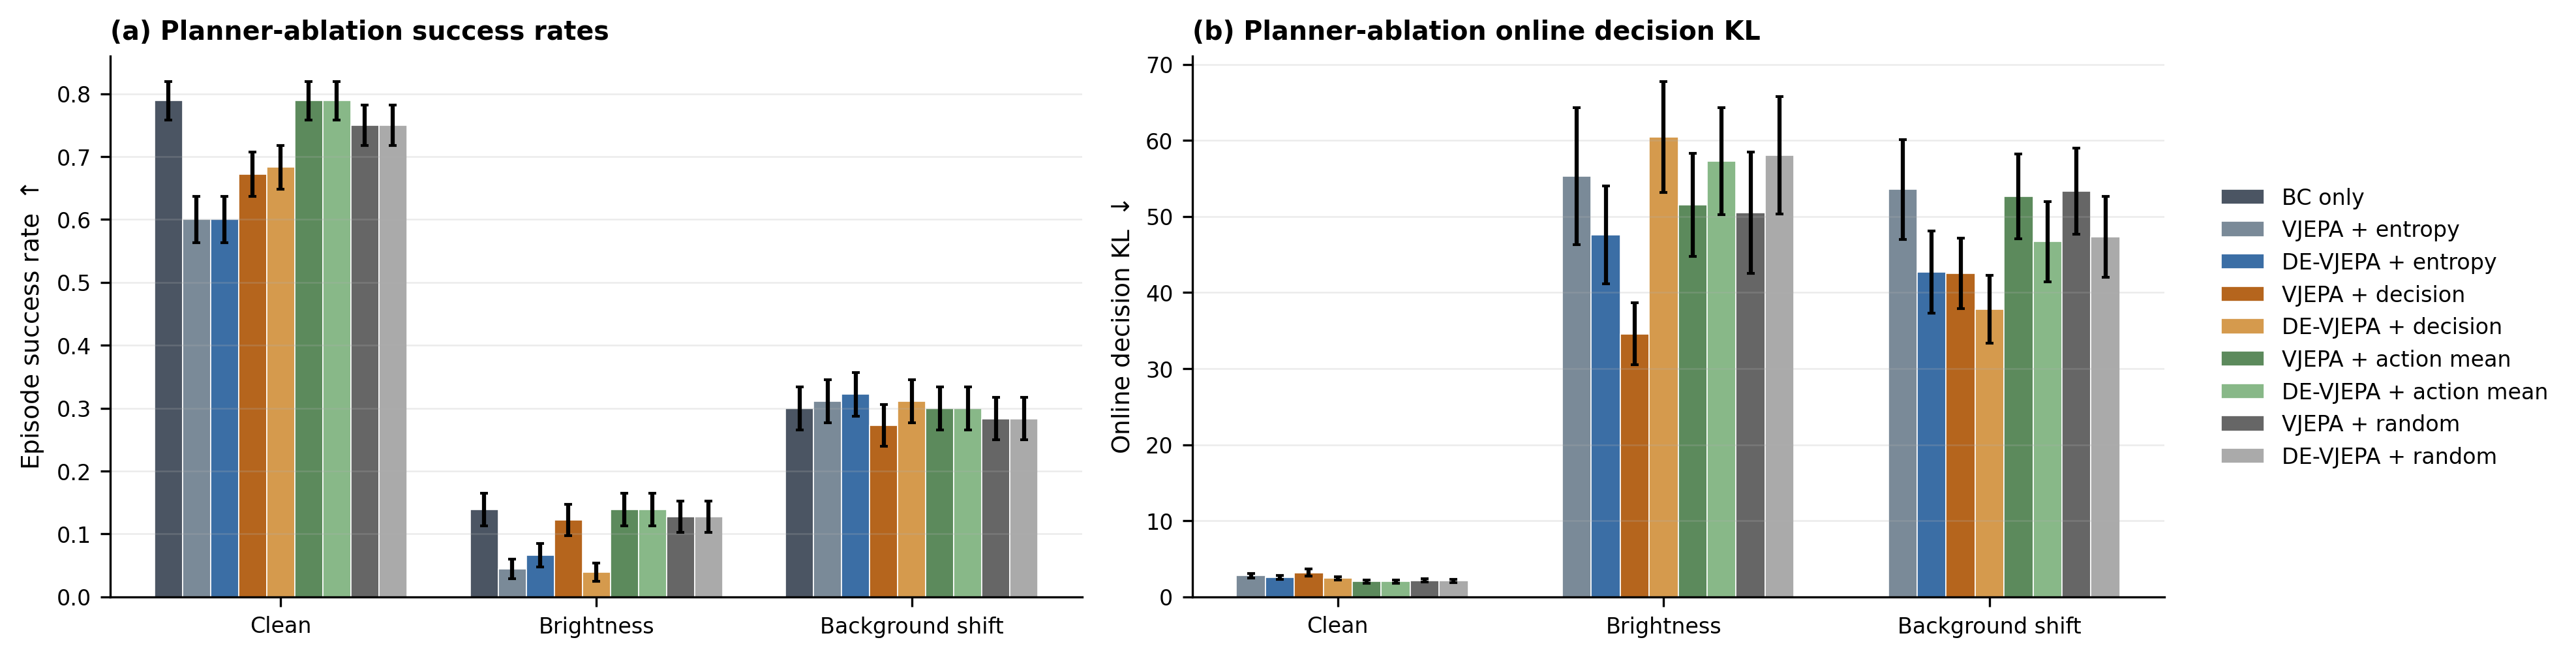
\includegraphics[width=\textwidth]{plots/planner_ablation_appendix.png}
\caption{Planner-ablation success (left) and online decision KL (right).
Improved online decision metrics do not imply improved task success. The
action-mean score remains almost exactly at the BC action and reproduces the
BC-only success rate.}
\label{fig:planner-ablation}
\end{figure*}

\subsection{Planner Ablation Statistical Results}

The paired unit is task--predictor-seed--visual-condition, yielding 27 units
overall and nine within each condition. DE-VJEPA versus VJEPA gives:
\begin{itemize}[leftmargin=1.5em,itemsep=1pt]
  \item entropy score: $+1.11$ success points,
  $p=0.680$, bootstrap CI $[-4.07,6.30]$;
  \item decision-consistency score: $-1.11$ points,
  $p=0.597$, CI $[-5.19,2.78]$;
  \item action-mean consistency: exactly $0.00$ points;
  \item random-candidate control: exactly $0.00$ points because candidate
  generation and random selection are paired and do not depend on the
  predictor.
\end{itemize}
No planner score establishes a DE-VJEPA success advantage over VJEPA.

Relative to BC-only, entropy scoring reduces VJEPA success by 9.07 points
($p=0.0215$) and DE-VJEPA success by 7.96 points ($p=0.0564$).
Decision-consistency scoring reduces VJEPA success by 5.37 points
($p=0.0341$) and DE-VJEPA success by 6.48 points ($p=0.00737$).
Random candidate selection reduces success by 2.22 points ($p=0.0202$).
Action-mean consistency has zero success difference from BC-only.

\paragraph{Action deviation explains the ordering.}
The mean root-mean-square action deviation from BC is approximately 0.12--0.15
for entropy and decision-consistency scoring, 0.107 for the random control, and
less than $6\times10^{-4}$ for action-mean consistency. Thus, the only planner
that matches BC success is also the planner that effectively declines to use
the world model. The experiment does not show that the predictors contain no
control-relevant information; it shows that the tested local scores do not
convert that information into better actions.

\paragraph{Condition-specific behavior.}
Entropy-scored DE-VJEPA is directionally better than entropy-scored VJEPA under
brightness (6.67\% versus 4.44\%) and background shift (32.22\% versus
31.11\%), but neither difference is significant. Decision consistency performs
poorly for DE-VJEPA under brightness (3.89\%) despite improved predicted
decision geometry elsewhere. This is evidence that minimizing local
distribution change can favor conservative or dynamically unhelpful actions.

\subsection{Autoregressive Multi-Step Diagnostic}

To separate planner failure from rapid model compounding error, trained
one-step VJEPA and DE-VJEPA predictors are rolled autoregressively over held-out
MetaWorld demonstration sequences. The predictor receives the recorded action
sequence but never receives future latents. Horizons $K\in\{1,3,5\}$ are scored
with the independent seed-7 BC evaluator. The final raw file contains 63,846
method--sample--horizon rows.

\begin{table}[t]
\centering
\caption{Multi-step diagnostic averaged across reach, button press, and drawer
open. Lower is better.}
\label{tab:multistep-final}
\resizebox{\columnwidth}{!}{%
\begin{tabular}{llrrr}
\toprule
\textbf{Method} & $\mathbf{K}$ & \textbf{Latent MSE} &
\textbf{Decision KL} & \textbf{Action MSE} \\
\midrule
VJEPA & 1 & \textbf{0.001336} & 0.3778 & 0.000289 \\
DE-VJEPA & 1 & 0.001545 & \textbf{0.3004} & \textbf{0.000267} \\
VJEPA & 3 & \textbf{0.003233} & 0.9050 & \textbf{0.000688} \\
DE-VJEPA & 3 & 0.003727 & \textbf{0.7888} & 0.000694 \\
VJEPA & 5 & \textbf{0.005170} & 1.5311 & \textbf{0.001124} \\
DE-VJEPA & 5 & 0.005886 & \textbf{1.3214} & 0.001138 \\
\bottomrule
\end{tabular}%
}
\end{table}

\begin{figure*}[!htbp]
\centering
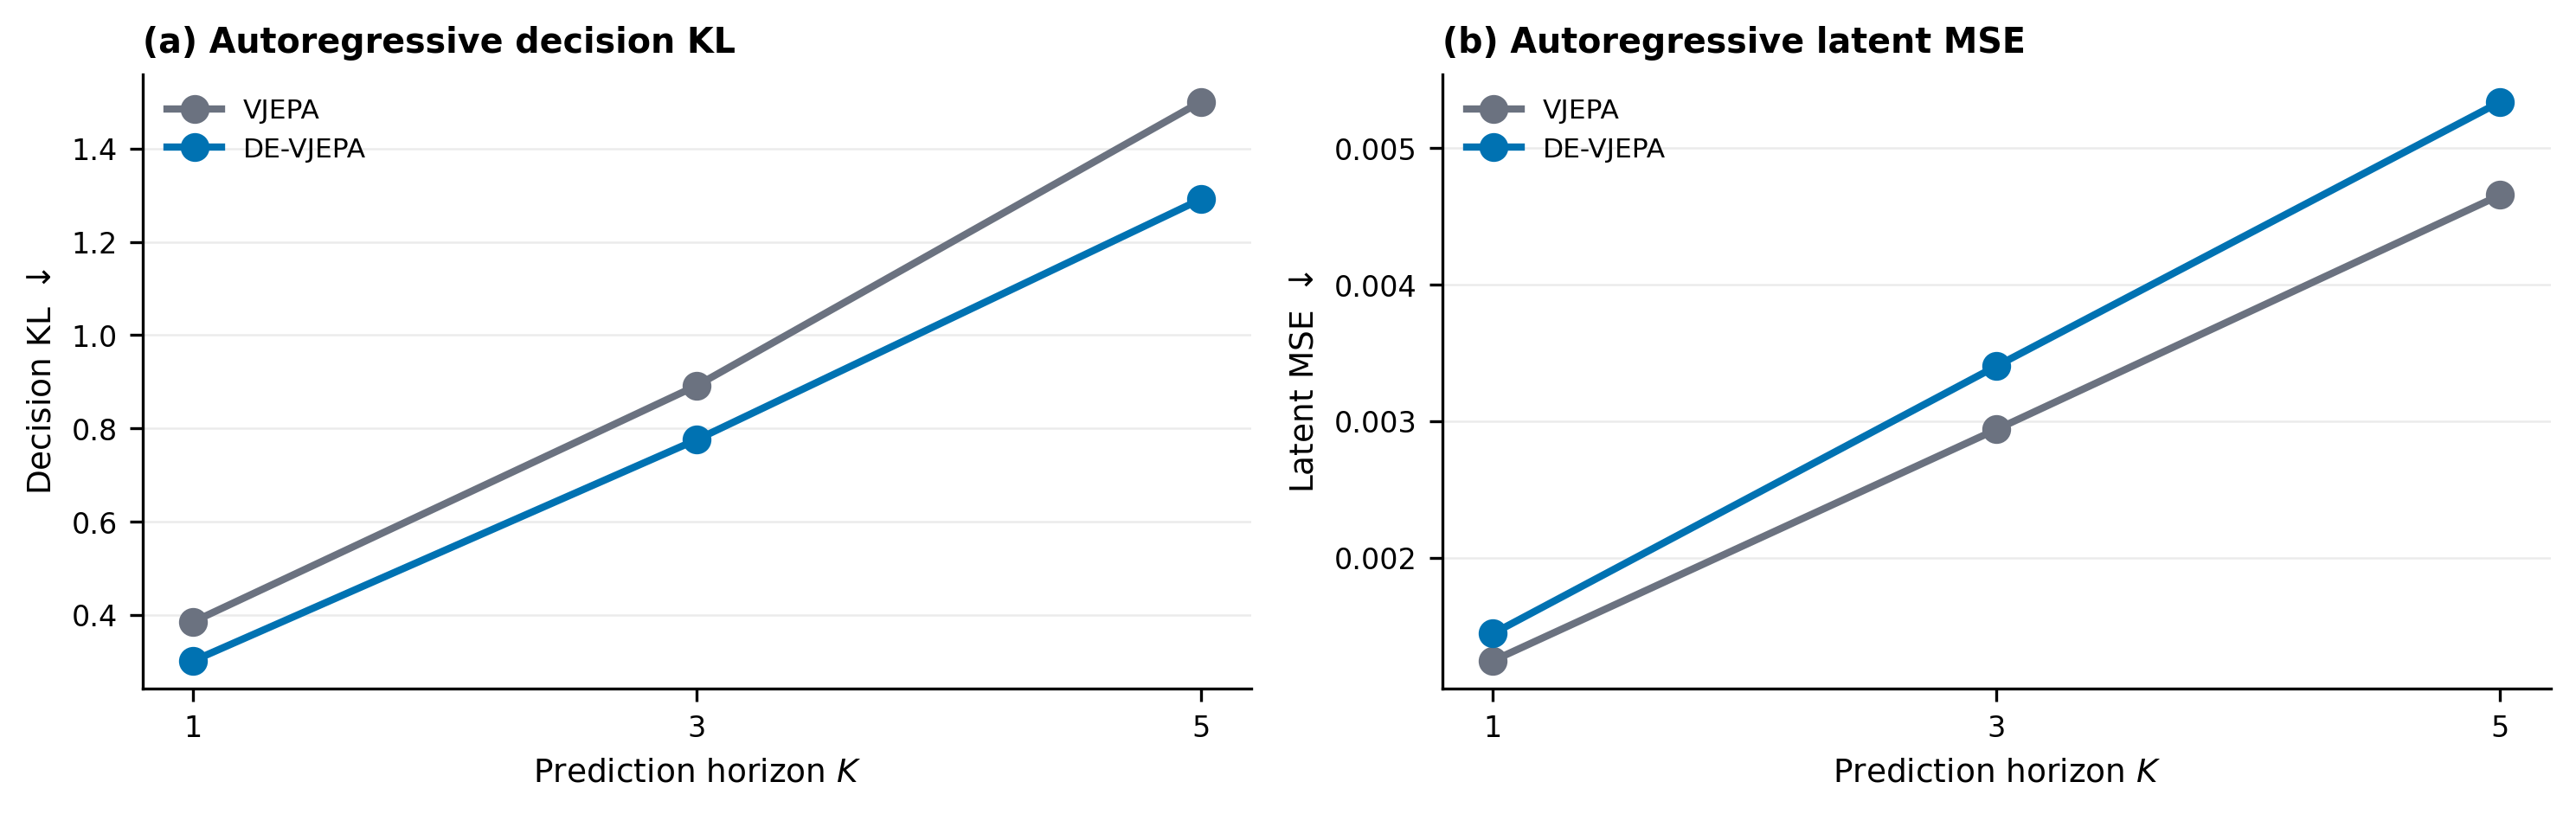
\includegraphics[width=\textwidth]{plots/multistep_appendix.png}
\caption{Autoregressive decision KL (left) and latent MSE (right). DE-VJEPA
maintains lower decision KL through horizon five while retaining the expected
latent-fidelity penalty.}
\label{fig:multistep-diagnostic}
\end{figure*}

DE-VJEPA reduces decision KL relative to VJEPA by approximately 20.5\% at
$K=1$, 12.8\% at $K=3$, and 13.7\% at $K=5$. Its mean decision-error slope is
also lower (0.255 versus 0.288 per prediction step). In contrast, DE-VJEPA
latent MSE is higher at every horizon, with latent-error slopes 0.001085 versus
0.000958. The decision advantage therefore weakens from its one-step maximum
but does not disappear by $K=5$.

\subsection{Revised Diagnosis of the Integration Gap}

The combined evidence rejects a simple explanation in which DE-VJEPA's
decision advantage immediately collapses under autoregressive prediction.
Instead:
\begin{enumerate}[leftmargin=1.6em,itemsep=2pt]
  \item DE-VJEPA preserves lower decision KL through five prediction steps.
  \item DE-VJEPA does not significantly beat VJEPA under any tested local
  candidate score.
  \item Entropy and decision-consistency scores underperform direct BC.
  \item Random perturbations also hurt, showing that candidate exploration
  itself has a measurable cost.
  \item Action-mean consistency matches BC only by producing negligible action
  deviations, not by exploiting predicted futures.
\end{enumerate}

The supported diagnosis is therefore: \emph{offline and multi-step
decision-preserving predictions are measurable, but local policy-consistency
objectives are not task-value objectives}. A useful next planner must score
long-horizon progress, reward, success probability, or value while controlling
model uncertainty. Appropriate next experiments are CEM/MPC over predicted
latents, a learned value head, multi-step DE training aligned to the planning
horizon, and policy improvement on imagined trajectories. Merely replacing one
local consistency score with another is unlikely to close the control gap.

\section{Supplementary Progress-Aware Planning Results}
\label{app:progress-planning}

\subsection{Progress-Head Validation}

The available MetaWorld demonstrations contain successful trajectories but do
not store reward-to-go or a task-specific distance target. We therefore train
a task-conditioned \emph{progress head}, not a value function, using
$y_t=t/(T-1)$. The MLP has two 512-unit hidden layers and is trained
independently with seeds 42, 1000, and 10000. Table~\ref{tab:progress-head-512}
reports validation statistics averaged over those seeds.

\begin{table}[t]
\centering
\caption{Validation of the 512-unit trajectory-progress head. Correlation is
with normalized time within a successful demonstration.}
\label{tab:progress-head-512}
\begin{tabular}{lrrr}
\toprule
\textbf{Task} & \textbf{MSE $\downarrow$} &
\textbf{Pearson $\uparrow$} & \textbf{Spearman $\uparrow$} \\
\midrule
All tasks & 0.000356 & 0.99794 & 0.99796 \\
Reach & 0.000990 & 0.99437 & 0.99431 \\
Button press & 0.000200 & 0.99897 & 0.99911 \\
Drawer open & 0.000078 & 0.99956 & 0.99956 \\
\bottomrule
\end{tabular}
\end{table}

The head easily reconstructs trajectory position. This validates the
implementation and provides a smooth planning score, but it does not establish
that the score measures causal task progress. In particular, a planner can
increase predicted trajectory time while moving to an off-demonstration
latent.

\subsection{One-Step Progress Planning}

The one-step study evaluates 4,860 episodes over three tasks, three predictor
seeds, three visual conditions, four action-deviation weights, and matched
VJEPA/DE-VJEPA predictors, with a shared BC-only control. At
$\alpha=0.1$, where actions remain close to BC, VJEPA and DE-VJEPA obtain
40.56\% and 40.93\% aggregate success, respectively. Their condition-level
success rates are 77.78/78.89\% on clean observations, 13.33/13.33\% under
brightness, and 30.56/30.56\% under background shift. The paired aggregate
difference is $+0.37$ percentage points ($p=0.161$).

Smaller penalties make the planner more active but less reliable. At
$\alpha=0.01$, DE-VJEPA improves over VJEPA under brightness by 9.44 points
(24.44\% versus 15.00\%), but the paired result is not significant
($p=0.231$), and clean success falls to 41.11\%. At $\alpha=0.3$, both
predictor planners nearly reproduce BC. The one-step result therefore does not
establish successful model-based control.

\subsection{Progress-Aware CEM/MPC}

CEM uses population 128, three refinement iterations, horizons
$H\in\{1,3,5\}$, and action penalties $\alpha\in\{0.01,0.1\}$. The complete
study contains 3,510 episodes. Table~\ref{tab:cem-progress-key} reports the
more stable $\alpha=0.1$ setting.

\begin{table}[t]
\centering
\caption{Progress-aware CEM success rates (\%) at $\alpha=0.1$. Each
method--horizon--condition cell contains 90 episodes.}
\label{tab:cem-progress-key}
\resizebox{\columnwidth}{!}{%
\begin{tabular}{llrrrr}
\toprule
\textbf{Method} & $\mathbf{H}$ & \textbf{Clean} &
\textbf{Brightness} & \textbf{Background} & \textbf{Overall} \\
\midrule
BC only & -- & 80.00 & 12.22 & 27.78 & 40.00 \\
\midrule
VJEPA+CEM & 1 & 76.67 & 13.33 & 30.00 & 40.00 \\
DE-VJEPA+CEM & 1 & 81.11 & 12.22 & 28.89 & 40.74 \\
VJEPA+CEM & 3 & 24.44 & 13.33 & 27.78 & 21.85 \\
DE-VJEPA+CEM & 3 & 26.67 & 26.67 & 28.89 & 27.41 \\
VJEPA+CEM & 5 & 18.89 & 15.56 & 25.56 & 20.00 \\
DE-VJEPA+CEM & 5 & 15.56 & 17.78 & 26.67 & 20.00 \\
\bottomrule
\end{tabular}%
}
\end{table}

At $H=1$, the two model-based planners are close to BC overall, and the
DE-VJEPA--VJEPA difference is $+0.74$ points ($p=0.537$). At $H=3$,
DE-VJEPA exceeds VJEPA by 5.56 points overall ($p=0.113$, paired 95\%
bootstrap CI $[-0.37,12.59]$) and by 13.33 points under brightness
($p=0.073$, CI $[2.22,24.44]$). The effect is directionally consistent with
the offline decision-preservation claim but does not cross the prespecified
significance threshold. At $H=5$, aggregate success is identical (20.00\%).

\subsection{Result and Remaining Test}

The progress-aware experiments refine, but do not overturn, the paper's
negative closed-loop conclusion. They show a potentially meaningful
DE-VJEPA advantage under horizon-three planning and brightness shift, while
also showing substantial clean-control degradation as the planning horizon
grows. The current evidence is compatible with two explanations: DE-VJEPA
provides a better latent rollout for moderate-horizon planning, or the observed
difference is sampling variation around a weak progress objective. The next
decisive experiment is horizon-matched $K=3$ predictor training followed by
the same $H=3$ CEM evaluation. Stronger-backbone evaluation is separately
required before attributing the offline result to representation-independent
decision geometry.

\begin{figure*}[!htbp]
\centering
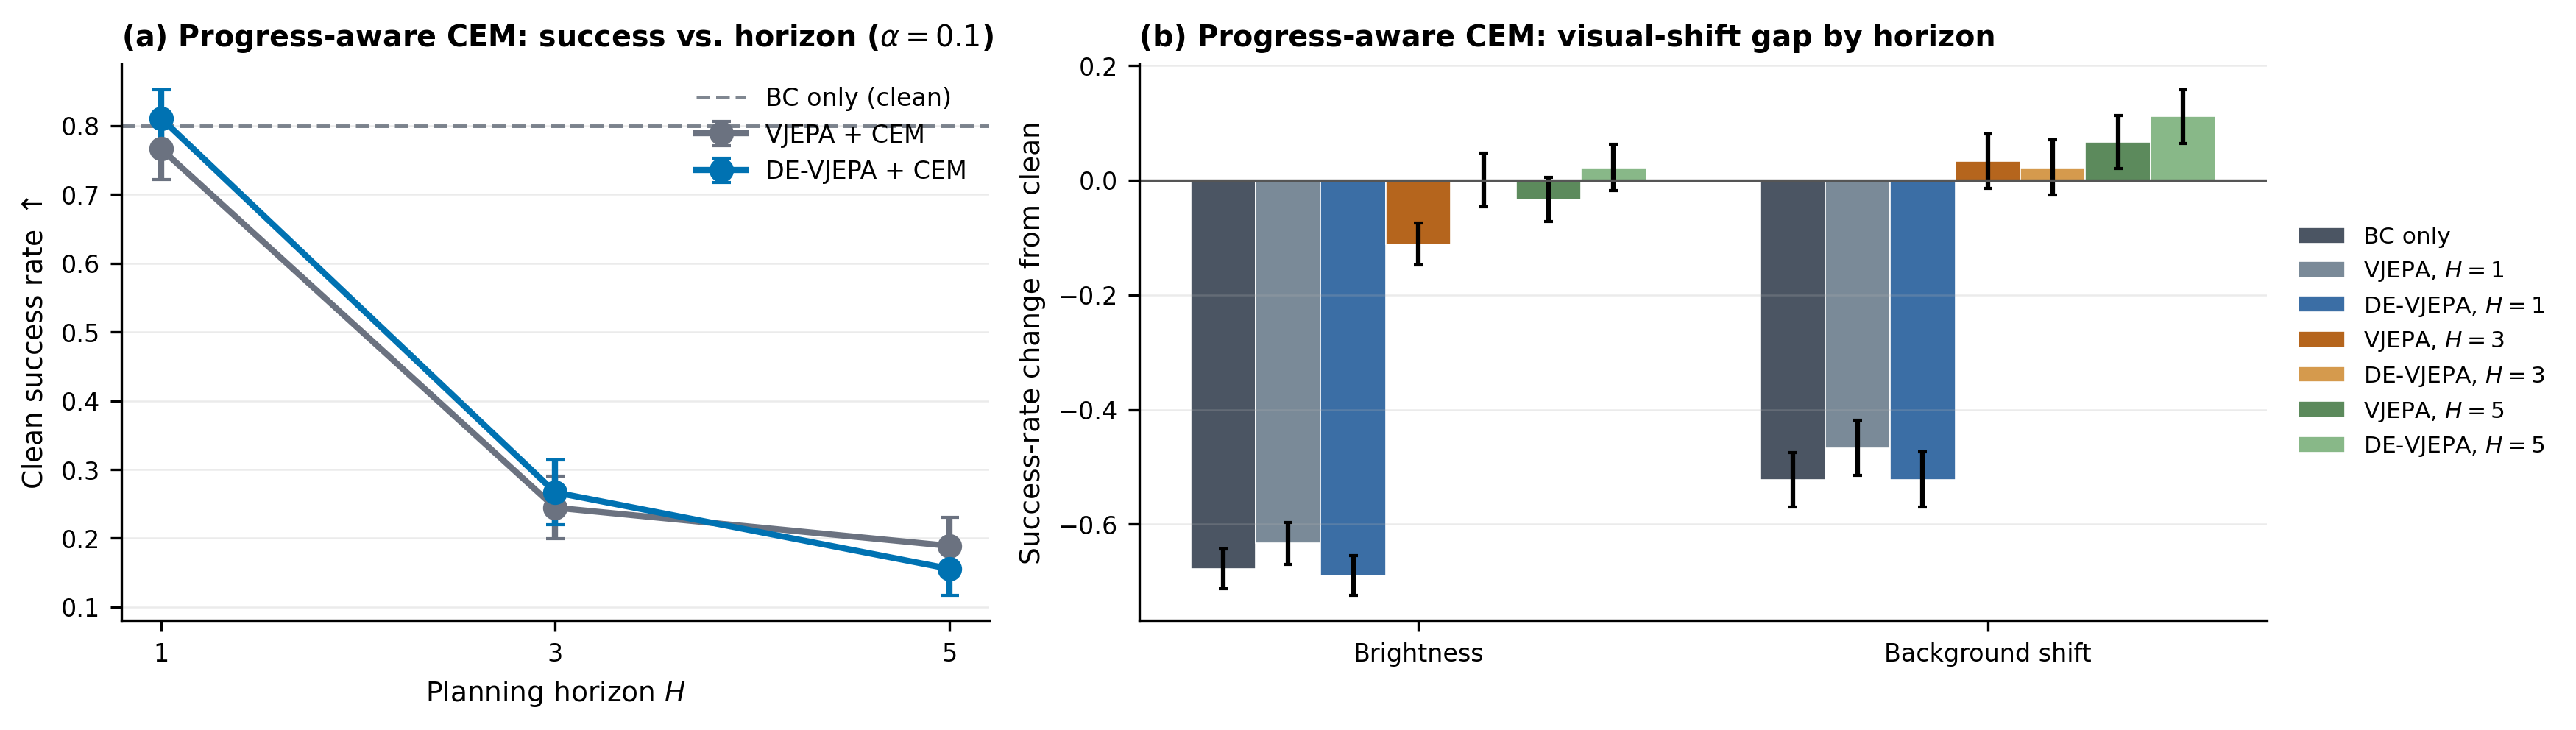
\includegraphics[width=\textwidth]{plots/cem_mpc_progress512_appendix.png}
\caption{Progress-aware CEM success by planning horizon (left) and visual
condition (right). Horizon three yields the largest directional DE-VJEPA
advantage, while longer planning does not improve aggregate success.}
\label{fig:cem-progress-512}
\end{figure*}

\section{Auxiliary Scaffolding Artifacts}
\label{app:scaffolding}

The release archive ships two scaffolding subsystems that were prototyped
during the closed-loop investigation but are deliberately \emph{not} part of
the load-bearing experimental evidence in this paper. We document them here
so the artifact inventory is self-explanatory and so follow-up work can pick
them up without rediscovering the wiring.

\paragraph{Value-head planner ($\tt value\_planner\_*$).} A scalar
state-value head trained on top of frozen VJEPA / DE-VJEPA features, intended
to provide a learned terminal cost for CEM rollouts (configs
\texttt{value\_head*.yaml} and \texttt{value\_planner*.yaml}; runner
\texttt{train\_value\_head.py}; summaries and figures named
\texttt{value\_planner*.\{csv,png\}}). On MetaWorld pilot tasks the head
converges and calibrates reasonably (smoke calibration plot), but combining
the head with CEM did not produce a closed-loop improvement that survived
seed averaging, so this branch was superseded by the progress-aware planner
reported in Appendix~\ref{app:progress-planning} (\texttt{cem\_mpc\_progress512}
artifacts). The full sweep CSVs and plots are retained as a negative-result
record and as a starting point for value-aware planning experiments that
share the same DE-VJEPA backbone.

\paragraph{DINOv2 backbone validation
($\tt backbone\_validation\_dinov2$, $\tt pilot\_dinov2$,
$\tt smoke\_dinov2.py$).} A backbone-substitution harness that swaps the
VJEPA encoder for a frozen DINOv2 ViT and reruns the offline decision-KL
pipeline. The harness exists to support the ``stronger-backbone evaluation
is separately required'' caveat noted above, but the corresponding training
sweep has not been launched in this submission. Only the launch scripts,
configs, and smoke test are shipped; no DINOv2 results table or figure is
included, and none of the main-text claims depend on this branch. We retain
the files so the substitution experiment is reproducible end-to-end as soon
as compute is available.

Both subsystems are isolated: removing the
\texttt{value\_planner*}/\texttt{value\_head*} and \texttt{*dinov2*} files
would not change any numeric result, table, or figure reported in
Sections~\ref{sec:experiments}--\ref{sec:limitations} of the main text.

\end{document}
